\section{Introduction}
\subsection{Présentation générale}
Les manœuvres de stationnement pouvant être parfois difficiles pour certains conducteurs, les constructeurs
automobiles proposent depuis maintenant quelques années une option de stationnement automatique sur leurs
véhicules. Cette fonctionnalité est permise par un système embarqué qui permet l’automatisation d’une manœuvre de stationnement (pour des places en créneau, épi ou bataille).

\begin{figure}[H]
\centering
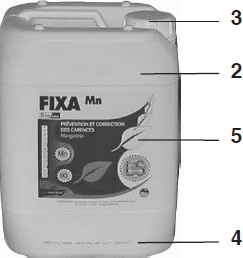
\includegraphics[width=.45\linewidth]{fig_00.png}
%\caption{ \label{fig_}}
\end{figure}

L’intervention du système de stationnement se fait sur la direction du véhicule : le système gère automatiquement l’orientation des roues avant du véhicule (et donc celle du volant). Quant au conducteur, il contrôle le
déplacement du véhicule (marche avant ou arrière) et la vitesse du véhicule avec la pédale d’accélération. Cette
vitesse est limitée et est supposée constante pendant la manœuvre.
Ce type d’aide au stationnement permet une meilleure précision de la manœuvre et un stationnement dans un
espace plus restreint en optimisant l’insertion du véhicule dans une place libre.
Les principaux éléments technologiques entrant en jeu dans cette automatisation des manœuvres de stationnement sont : le calculateur du véhicule, la motorisation de la direction du véhicule et les capteurs à ultrasons (généralement entre 4 et 6 capteurs à l’avant et à l’arrière).

\begin{figure}[H]
\centering
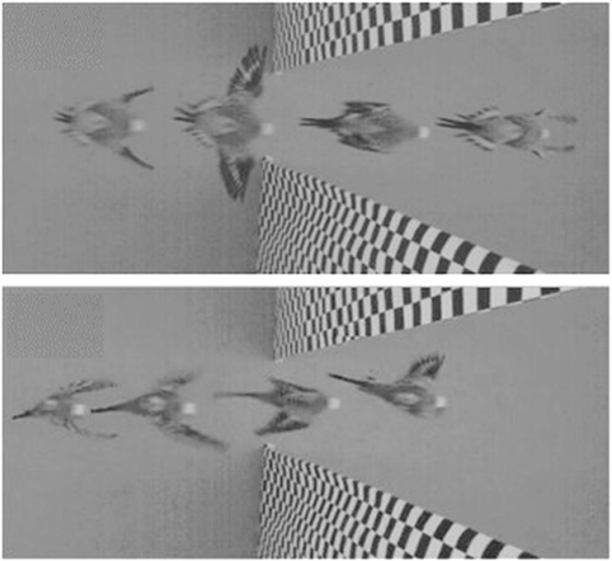
\includegraphics[width=.45\linewidth]{fig_01.png}
\caption{Détection par ultrasons (4 capteurs) \label{fig_01}}
\end{figure}

La procédure d’insertion automatisée du véhicule dans une place de stationnement, du point de vue du conducteur, est décrite par la \autoref{fig_02} dans le cas d’une insertion en créneau parfaitement exécuté. Sur la figure, le
véhicule est équipé de 4 capteurs à ultrasons à l’avant et à l’arrière.

Lorsque le conducteur voit une place libre devant lui, il active le stationnement automatique par l’appui d’un
bouton dédié sur son tableau de bord. La voiture est parallèle au trottoir et se déplace dans le sens normal de
la marche (repère 1 \autoref{fig_02}).

Le déclenchement du stationnement automatique a pour conséquence la détection de l’emplacement libre par
les capteurs ultrasons équipant la voiture lorsque celle-ci se déplace (repère 2 \autoref{fig_02}).
Si la place de stationnement est suffisamment longue et profonde alors le conducteur est prévenu que la manœuvre
est possible par un voyant lumineux situé sur son tableau de bord. Le conducteur doit alors arrêter son véhicule
(repère 3 \autoref{fig_02}) et mettre la boite de vitesses au point mort (position neutre).


\begin{figure}[H]
\centering
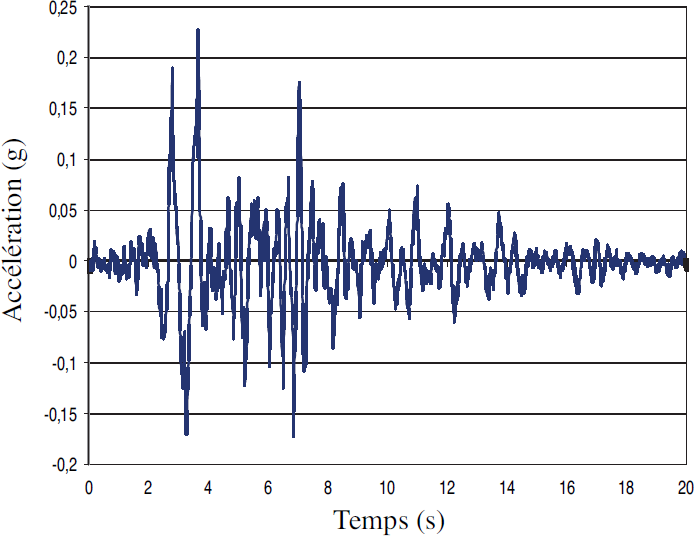
\includegraphics[width=.9\linewidth]{fig_02.png}
\caption{Manoeuvre d’insertion en créneau dans une place de stationnement \label{fig_02}}
\end{figure}

Un signal sur le tableau de bord invite alors le conducteur à passer la marche arrière et à appuyer sur la pédale
d’accélération afin que le véhicule commence la manœuvre (repères 4 et 5 \autoref{fig_02}). Pendant la manœuvre le
conducteur ne touche pas le volant.
Le processus d’automatisation de l’insertion du véhicule dans une place de stationnement en créneau suit un
algorithme dont l’action dépend du type de manœuvre, de l’espace de stationnement et de la géométrie du
véhicule. Cet algorithme gère :
\begin{itemize}
\item la détection d’une place libre suffisamment longue et profonde pour la manœuvre ;
\item le calcul de la trajectoire à suivre ;
\item la commande de la direction du véhicule.
\end{itemize}
Les exigences que le système de stationnement doit respecter sont décrites en figure \autoref{fig_26}.

\subsection{Problématique et organisation de l’étude}
Lors d’un stationnement en créneau, c’est la phase d’insertion du véhicule dans la place envisagée qui va
conditionner la réussite du stationnement et le nombre de manœuvres permettant d’atteindre une position
correcte de stationnement.

\begin{obj}
L’étude proposée a pour objectif de définir et de valider les conditions et les modèles à implanter dans
un algorithme de stationnement automatique afin qu’une manœuvre d’insertion de type créneau dans
une place de stationnement soit réussie et qu’elle atteigne les niveaux de performance attendus.
\end{obj}

L’étude est limitée à une manœuvre en créneau dont la position finale est définie repère numéro 5 sur la \autoref{fig_02}.
La manœuvre d’insertion en stationnement doit être réalisée en une fois. Si l’insertion est réussie alors la position
finale de stationnement sera, dans un second temps, facilement atteinte par une légère avance du véhicule pour
être centré dans la place de stationnement.

Dans un premier temps l’étude portera sur le stationnement automatique d’un véhicule réel. Le travail mené en
début de sujet pour un véhicule réel pouvant être transposé (à l’échelle près) à tout type de véhicule roulant,
le support technique de l’étude sera dans un second temps une voiture radio commandée (elle sera présentée
ultérieurement dans l’étude). Ce choix est justifié par le fait qu’il n’est pas possible de réaliser des essais sur un
véhicule réel et que les choix technologiques de la commande de direction ne sont pas rendus accessibles par les
constructeurs automobiles.


\section{Détection de l’environnement et prédiction de la trajectoire de
stationnement}

La phase pendant laquelle le véhicule circule parallèlement à une place libre est primordiale car elle correspond
à la phase de détection de l’emplacement de stationnement. Cette détection doit permettre de vérifier la compatibilité de l’emplacement détecté avec la manœuvre automatisée et d’identifier dans l’environnement du véhicule
des repères géométriques à partir desquels l’algorithme pourra établir la trajectoire à suivre.
Ces deux tâches sont possibles grâce aux capteurs de proximité à ultrasons équipant le véhicule (\autoref{fig_02}) et à
l’exploitation de leurs signaux.

\begin{obj}
Les objectifs de cette partie sont de déterminer les conditions à implanter dans l’algorithme de stationnement pour la validation d’une place libre et de caractériser la géométrie de la trajectoire à
suivre pour mener avec succès la manœuvre de stationnement. Cette trajectoire servira de consigne à
l’algorithme pour son action sur la direction du véhicule.
\end{obj}

\subsection{Détection et caractérisation d’une place libre (exigence 1.4)}
\begin{obj}
L’objectif est de caractériser les conditions définissant une place compatible avec la manœuvre de
stationnement.
\end{obj}

Lors du fonctionnement du véhicule tous les capteurs sont actifs, mais tous ne sont pas forcément exploités
pour la manœuvre automatique. Ainsi on distingue les capteurs dont les signaux peuvent être exploités par
l’algorithme de stationnement et ceux dont le signal sera exploité pour la sécurité (des passagers, des autres
usagers de la route et des piétons lors de la manœuvre du véhicule).

\question{À partir du diagramme des exigences (\autoref{fig_26}) et de la \autoref{fig_02}, identifier le ou les capteurs à ultrasons pouvant participer au respect de l’exigence 1.4. Faire de même pour l’exigence 1.6.1.}
\ifprof
\begin{corrige}
Pour trouver une place de stationnement à droite, seuls les capteurs positionnés à droite sont nécessaires. 
\begin{itemize}
\item Exigence 1.4 :
\begin{itemize}
\item $L_p \geq L_v + 2 \times 0,5 $ (Longueurs) : capteurs b et d;
\item $l_p \geq l_v + 2 \times 0,15 $ (largeurs) : a et c. 
\end{itemize} 
\end{itemize}

\begin{itemize}
\item Exigence 1.6.1 : l'utilisateur doit contrôler le déplacement du véhicule tous les capteurs ultrasons doivent être utilisés.
\end{itemize}

\end{corrige}
\else
\fi

Dans la réalité, le signal du capteur latéral côté passager (capteur a \autoref{fig_03}) est suffisant pour détecter une
place de stationnement suffisamment spacieuse. Le signal fourni par le capteur a va permettre de savoir si la
place de stationnement envisagée par le conducteur est compatible avec la manœuvre, mais va aussi permettre
de définir certains repères géométriques de l’environnement. Ces repères géométriques vont servir de référence
pour l’élaboration de la trajectoire à suivre pour réaliser le stationnement en créneau.


\begin{figure}[H]
\centering
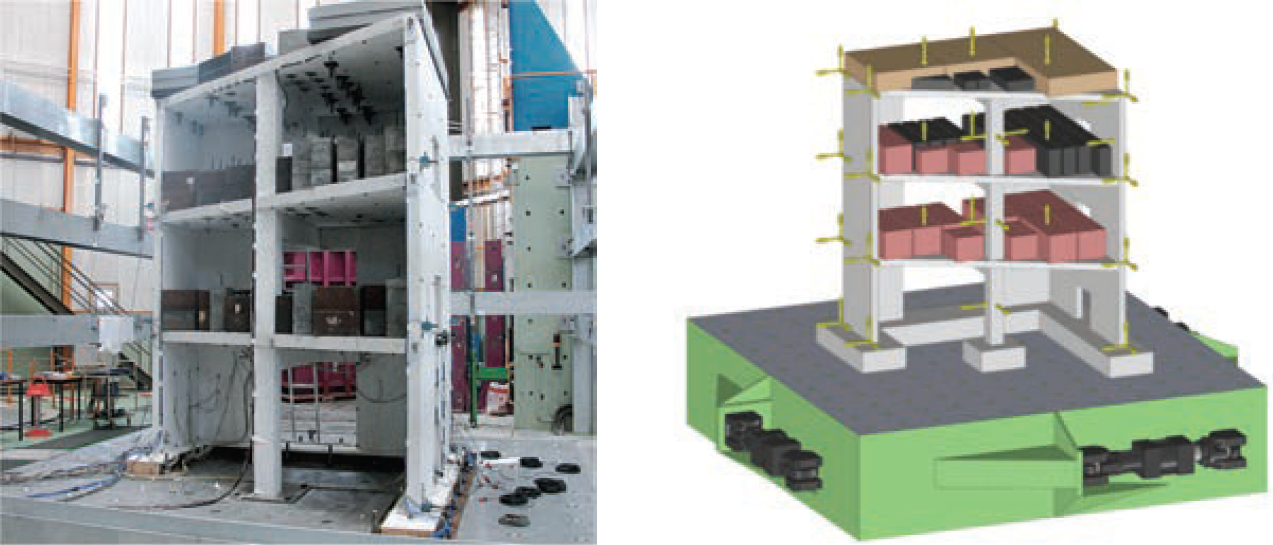
\includegraphics[width=.45\linewidth]{fig_03.png}
\caption{Phase de détection d’une place libre \label{fig_03}}
\end{figure}

Le type de capteur utilisé est un capteur de proximité à ultrasons (\autoref{fig_04}). Ce type de capteur possède une
membrane qui émet une onde ultrasonore par vibrations. La distance $d$ entre un capteur et un obstacle est
déduite du temps $T_e$ d’aller et retour de l’onde qui est réfléchie par l’obstacle puisque la vitesse du son dans
l’air est connue : $V_s = \SI{340}{m.s^{-1}}$.

\begin{figure}[H]
\centering
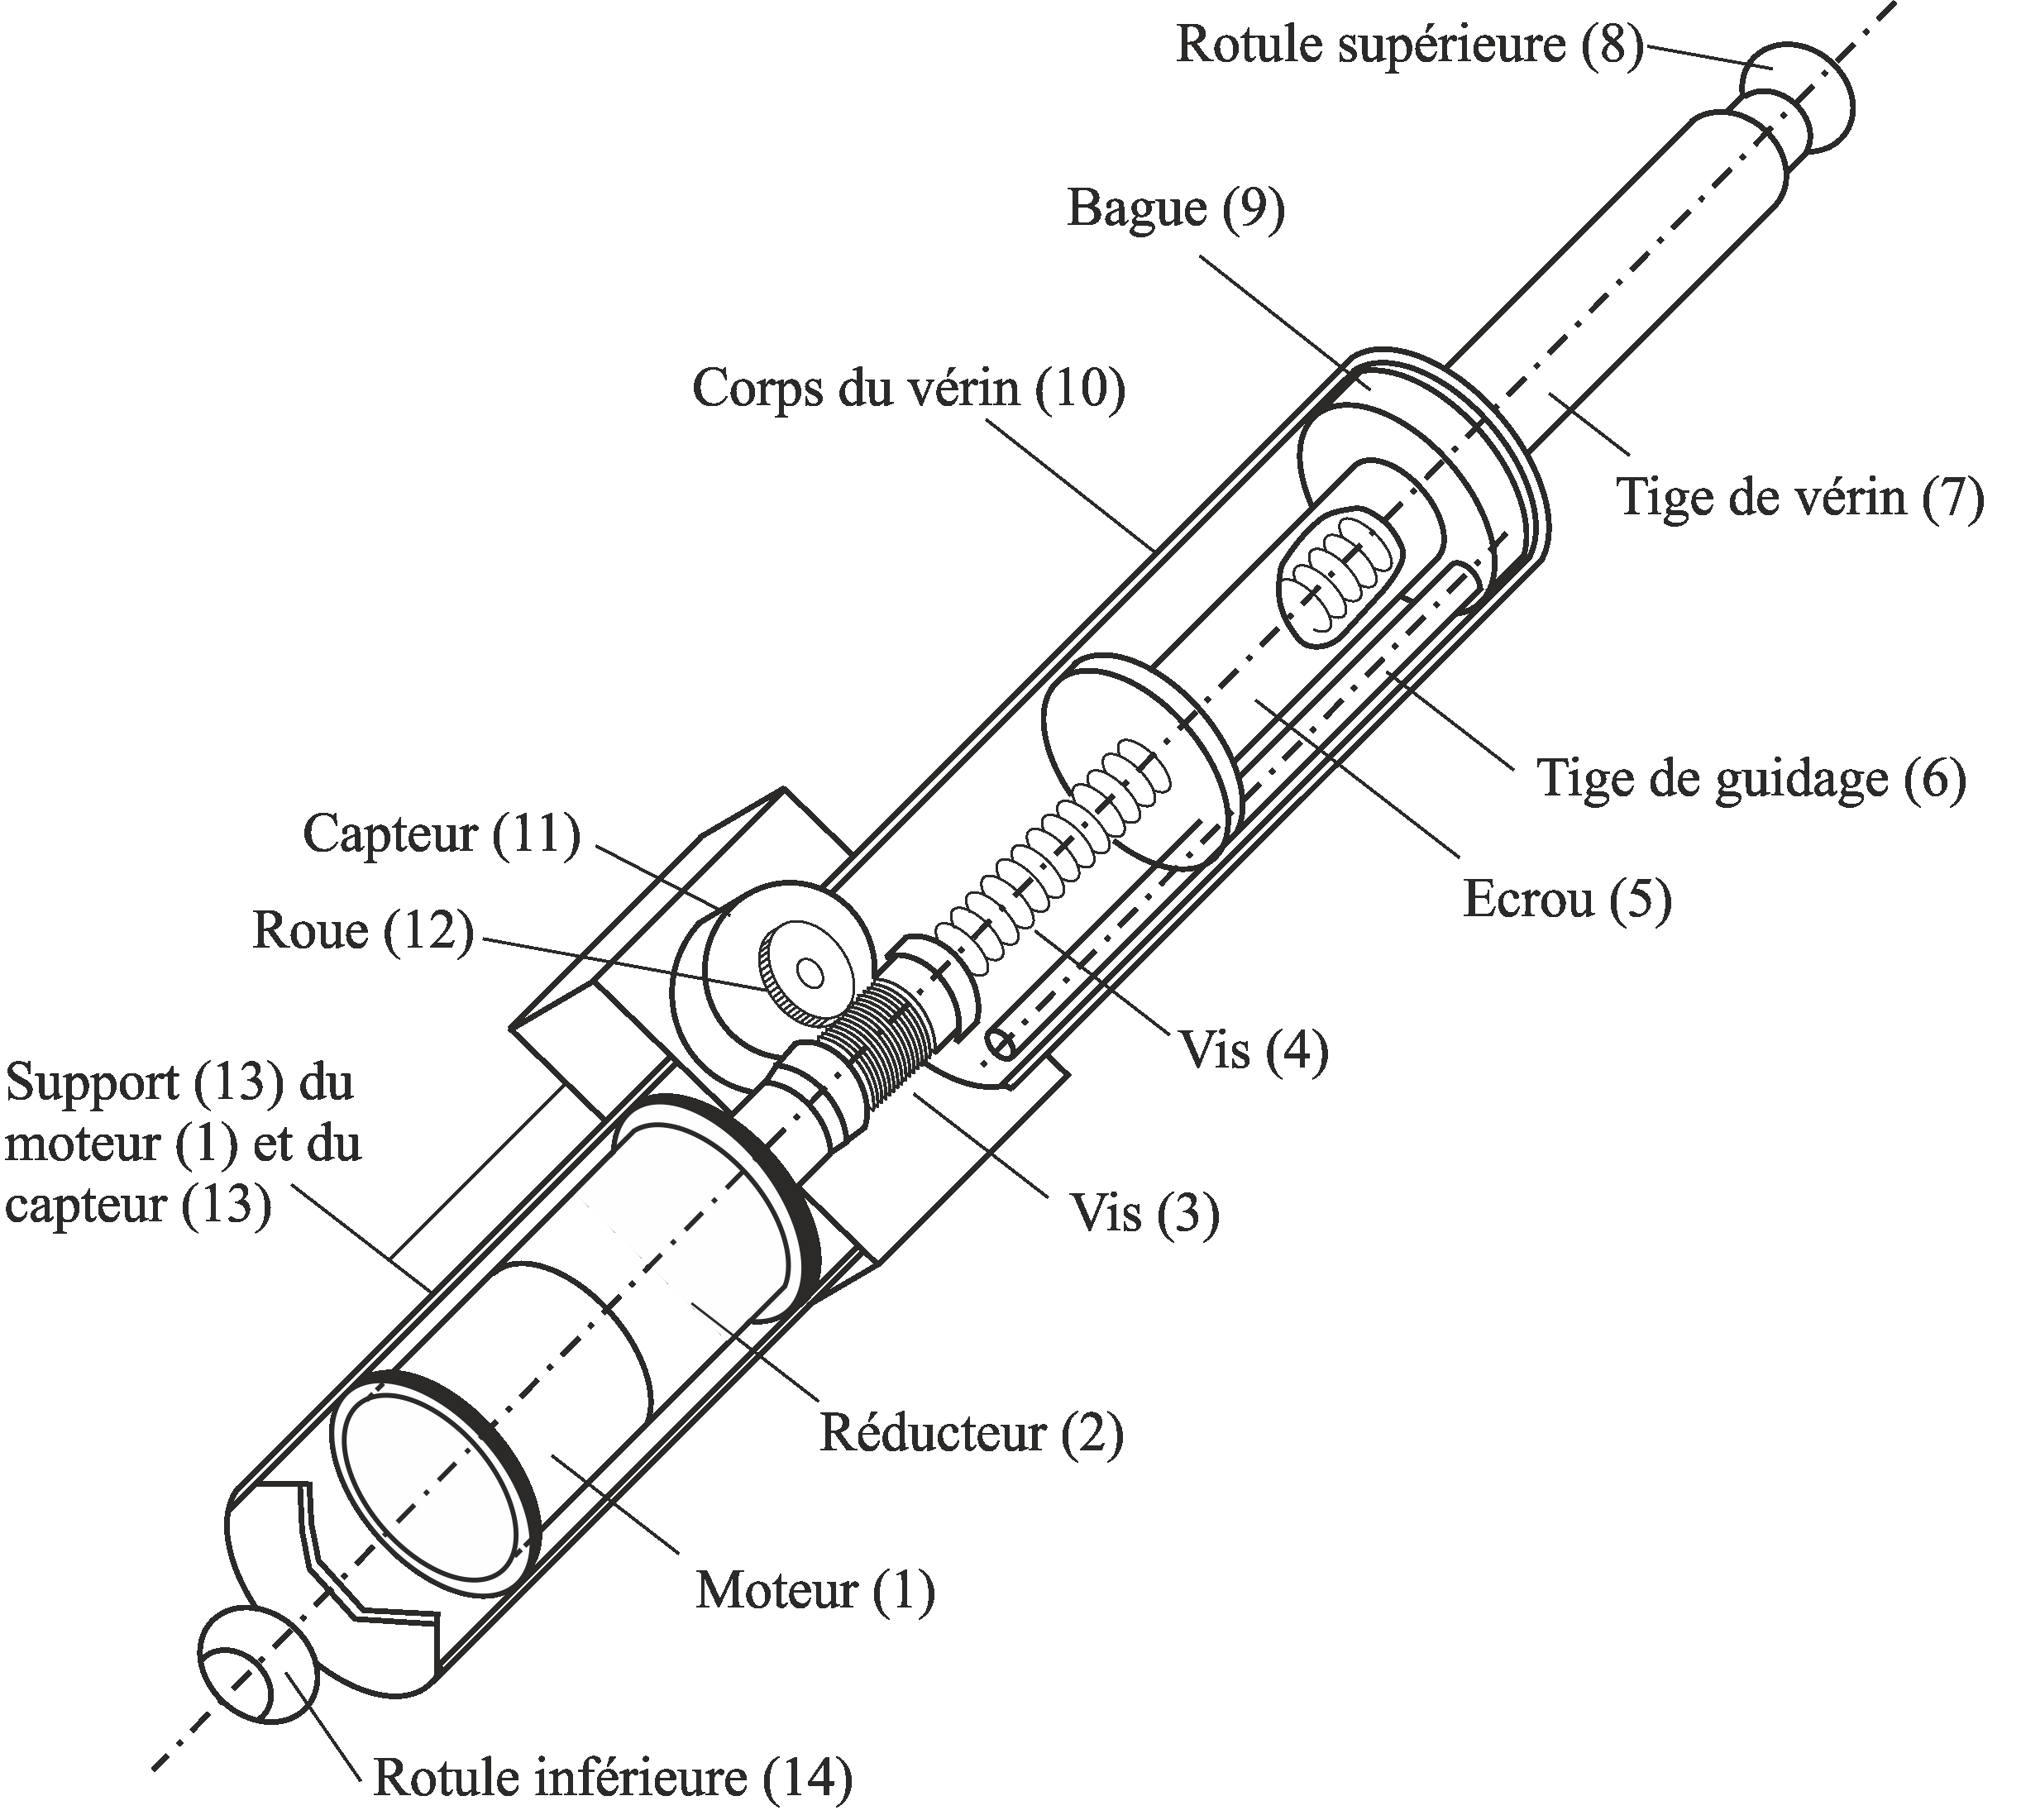
\includegraphics[width=.7\linewidth]{fig_04.png}
\caption{Principe du capteur de proximité \label{fig_04}}
\end{figure}

Ainsi au niveau du capteur de proximité, l’information exploitable est le temps $T_e$
entre l’émission et la réception
du signal (écho) émis par le capteur. C’est l’acquisition de $T_e$ qui servira dans l’algorithme pour l’identification
d’une place libre et pour la caractérisation de la trajectoire à suivre.

La \autoref{fig_05} représente le profil de vitesse du véhicule lorsque ce dernier longe une place libre. Le temps $T_a$
représente l’instant où le temps $T_e$ augmente brusquement (ce qui correspondrait au point $A$ \autoref{fig_03}). Le temps
$T_b$
correspond au moment où $T_e$ diminue brusquement (ce qui correspondrait au point B \autoref{fig_03}).

\begin{figure}[H]
\centering
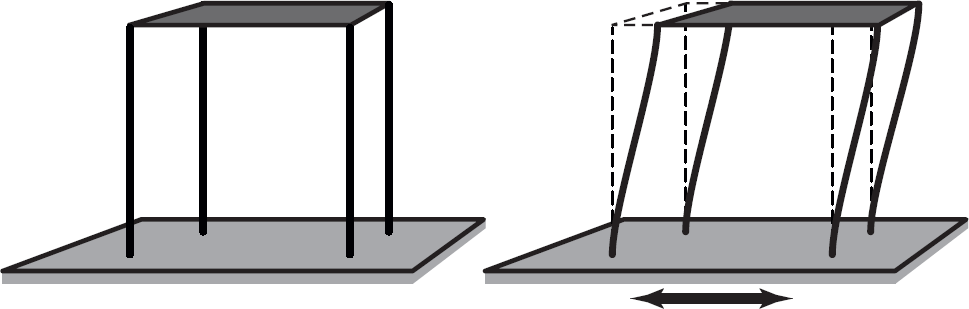
\includegraphics[width=.7\linewidth]{fig_05.png}
\caption{Profil de vitesse du véhicule lors des phases 1, 2 et 3 de la figure \ref{fig_05} \label{fig_05}}
\end{figure}

Lors de la phase de détection le véhicule avance à une vitesse $V_d$ constante et connue (information déduite de
capteurs situé au niveau des roues). La longueur du véhicule notée $L_v$
est également connue comme tous les
paramètres géométriques du véhicule.

Le fait de relever $\Delta T_p = T_b - T_a$ au niveau du capteur \textbf{a} permet de déterminer la longueur de la place et de vérifier qu’elle est compatible avec la manœuvre.

\question{Déterminer la condition que la grandeur $\Delta T_p$ doit vérifier pour que la longueur $L$ d’une place de stationnement respecte l’exigence 1.4. Cette condition est fonction de $V_d$ et $L_v$.}
\ifprof
\begin{corrige}
À vitesse constante, $V_d = \dfrac{L}{\Delta T_p}$. Or d'après l'exigence 1.4, $L \geq L_v + 2\times 0,5$ soit 
$V_dT_p \geq L_v + 1$ et $T_p \geq\dfrac{ L_v + 1}{V_d}$.
\end{corrige}
\else
\fi

Lorsque la voiture longe la place libre (entre les repères A et B \autoref{fig_03}), c’est la valeur maximale de $T_e$ relevée
lors du déplacement qui permet de savoir si la largeur de la place est suffisante pour la manœuvre. Cette largeur
est notée $e$ (\autoref{fig_03}) et la largeur du véhicule est notée $e_v$. La grandeur $D$ désigne la distance latérale par rapport aux véhicules déjà stationnés (\autoref{fig_03}).

\question{Déterminer la condition sur le temps $T_e$ pour que la largeur d’une place de stationnement respecte
l’exigence 1.4.}
\ifprof
\begin{corrige}
D'après l'exigence 1.4, $e>e_v + 0,15$.
Dans ces conditions, $T_e = \dfrac{2e}{V_s}$.
On a donc $\dfrac{T_e V_s}{2}>e_v + 0,15$ et $T_e>2\dfrac{e_v + 0,15}{V_s}$.


\end{corrige}
\else
\fi


Les conditions de longueur et de largeur d’une place de stationnement étant vérifiées, les distances $L$ et $e$ étant déduites des mesures, ces deux dernières grandeurs sont désormais des données implantables dans l’algorithme de stationnement. Le fait de connaitre en temps réel la vitesse du véhicule donne aussi la possibilité de connaitre la position du véhicule à partir d’un instant de référence tel que $T_a$. Il est donc maintenant considéré que la
position du point $A$ par rapport au véhicule est une donnée.

Une place de stationnement libre étant acceptée pour la manœuvre et sa géométrie (longueur, largeur, position
des obstacles) étant connue, il reste à caractériser la trajectoire à suivre pour la manœuvre.

\subsection{Trajectoire à suivre pour le stationnement (exigence 1.2)}

\begin{obj}
L’objectif est de déterminer les paramètres géométriques à implanter dans l’algorithme de stationnement afin d’y définir la trajectoire à suivre pour le stationnement.
\end{obj}

\subsubsection{Caractérisation de la trajectoire à suivre}
Une fois que le véhicule a longé une place et qu’il est à l’arrêt (position 3 \autoref{fig_02}) la manœuvre de type créneau
débute par une phase de recul rectiligne jusqu’à ce que le train arrière soit au niveau de l’extrémité arrière du
véhicule déjà stationné (point $B$ \autoref{fig_06}). Toujours en recul, il s’en suit le braquage des roues (dans un sens
puis l’autre) pour l’insertion dans la place libre.

La trajectoire du véhicule est définie par celle du point $F$, centre du train arrière (\autoref{fig_06}). La trajectoire
« idéale~» de $F$ est donc une portion linéaire jusqu’au point $O$ suivie de deux arcs de cercles identiques (sur les cercles $C_1$ et $C_2$) tangents en un point $P$. Ce dernier est le point où le véhicule fait un angle de 45\degres par rapport
au trottoir.

Le point $O$ est défini à partir de la longueur $L$  de la place de stationnement, des dimensions du véhicule et de
la distance $D$ de ce dernier avec le véhicule déjà stationné en amont de la place libre.

Le \autoref{tab_01} précise les paramètres géométriques qui caractérisent la trajectoire du véhicule pendant la manœuvre de stationnement.

\question{Parmi tous les paramètres géométriques définis dans le \autoref{tab_01} ainsi que sur la \autoref{fig_06}, identifier
ceux qui sont propres au véhicule et ceux qui se déduisent directement des informations des capteurs à ultrasons.
Que reste-t-il donc à déterminer afin que la géométrie de la trajectoire du point $F$ soit définie ?}
\ifprof
\begin{corrige}
\end{corrige}
\else
\fi

\begin{figure}[H]
\centering
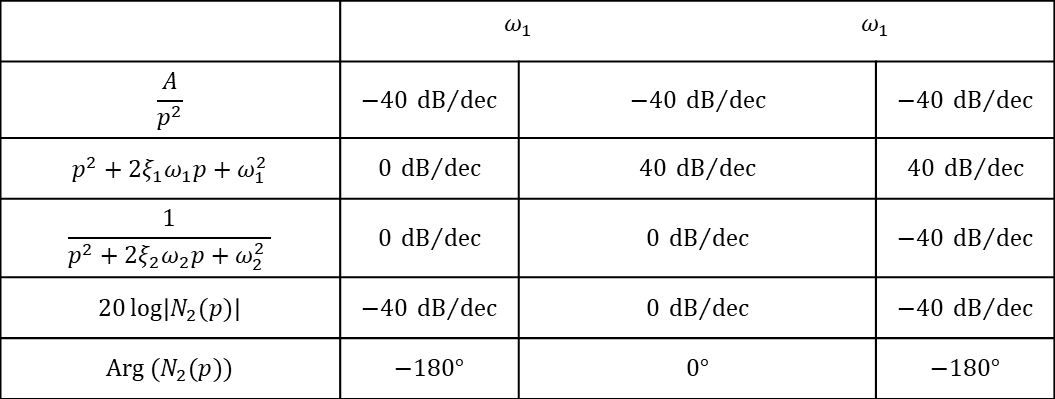
\includegraphics[width=\linewidth]{fig_06.png}
\caption{Trajectoire à suivre pour la manoeuvre \label{fig_06}}
\end{figure}

\begin{table}
\begin{itemize}
\item Paramètres de la place de stationnement :
\begin{itemize}
\item $L$ longueur de la place libre ;
\item $e$ largeur de la place libre.
\end{itemize}
\item Autres paramètres géométriques :
\begin{itemize}
\item $D$ distance latérale par rapport au véhicule déjà stationné ;
\item $L_F$ distance train arrière/extrémité arrière du véhicule ;
\item $R$ rayon des cercles $C_1$ et $C_2$ composant la trajectoire ;
\item $L_a$ distance entre l’arrière du véhicule en manœuvre et du véhicule placé derrière ;
\item $e_v$ largeur du véhicule en manœuvre ;
\item $d_r$ distance latérale entre le véhicule stationné et tout obstacle limitant la largeur de la place de stationnement.
\end{itemize}
\end{itemize}
\caption{Définition des paramètres géométriques qui caractérisent la trajectoire \label{tab_01}}
\end{table}

\begin{itemize}
\item $\rep{0} \repere{O}{x_0}{y_0}{z_0}$ est un repère défini au point $O$. 
\item Les points $O_1$ et $O_2$ sont respectivement les centres des cercles $C_1$ et $C_2$.
\item Le point $P$ est milieu de $[O_1 O_2]$.
\item Les cercles $C_1$ et $C_2$ sont de même rayon $R$.
\item La position du point $F$ est repérée par un angle $\theta_1(t)$ (\autoref{fig_07}) dans le repère
$\repere{O_1}{x_0}{y_0}{z_0}$ et par un angle $\theta_2(t)$ (\autoref{fig_07}) dans le repère $\repere{O_2}{x_0}{y_0}{z_0}$.
\item Le point $F_0$ correspond à la position initiale du point $F$ et $F_f$ à celle de la position finale lors de la phase d’insertion.
\end{itemize}


\begin{figure}[H]
\centering
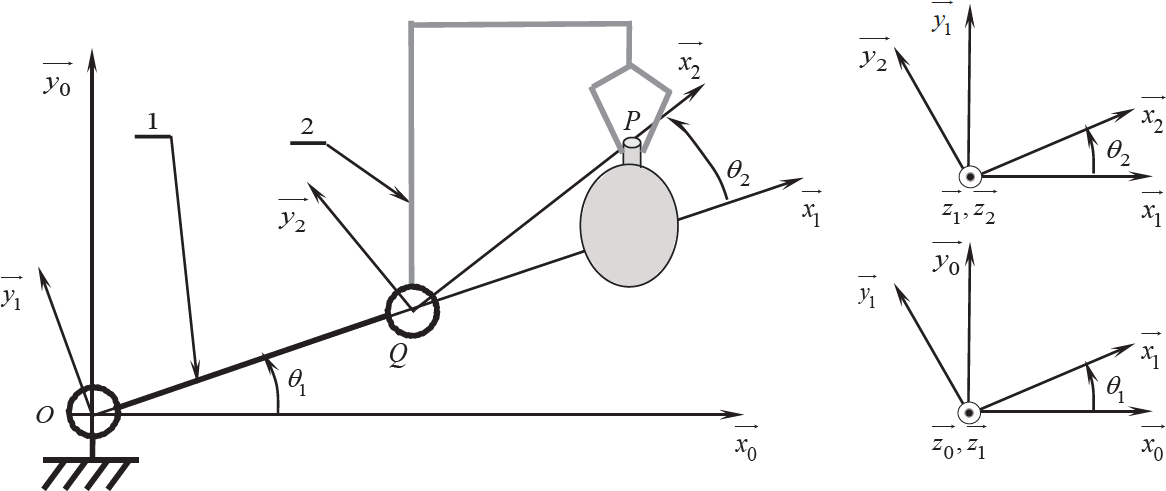
\includegraphics[width=.75\linewidth]{fig_07.png}
\caption{Trajectoire du point $F$ lors de l’insertion dans la place vacante \label{fig_07}}
\end{figure}

%Q5
\question{Les coordonnées du point $P$ dans le repère $\rep{0}$ sont notées $x_p$
et $y_p$ : $\vect{OP}=x_P\vect{x_0}+y_P\vect{y_0}$. Déterminer
l’expression de $x_P$ et $y_P$ en fonction des paramètres géométriques $L$, $e$, $L_F$, $d_r$, $L_a$ et $D$. Le rayon $R$ n’étant pas encore déterminé, il ne doit pas apparaitre dans les expressions de $x_P$ et $y_P$.}
\ifprof
\begin{corrige}
On a $x_P = \dfrac{1}{2} \vect{OF_f}\cdot \vect{x_0} = \dfrac{1}{2}\left(L-L_a - L_f\right)$.

De plus $y_P = \dfrac{1}{2} \vect{OF_f}\cdot \vect{y_0} = \dfrac{1}{2}\left(\dfrac{e_v}{2}+D+e - d_r - \dfrac{e_v}{2} \right)=\dfrac{1}{2}\left(D+e - d_r \right)$ .
\end{corrige}
\else
\fi

%Q6
\question{Déterminer l’expression de $R$ en fonction de $L$, $L_a$ et $L_F$ qui permettra de définir le cercle $C_1$ (et donc le cercle $C_2$).}
\ifprof
\begin{corrige}
On a $\vect{OP}=\vect{OO_1}+\vect{O_1P}$. 
%En projetant sur $\vect{y}$, on a 
%$y_P = R - R\dfrac{\sqrt{2}}{2}$ soit 
%$\dfrac{1}{2}\left(D+e - d_r \right)= R\dfrac{2-\sqrt{2}}{2}$ soit $R=\dfrac{D+e - d_r }{2-\sqrt{2}}$.

En projetant sur $\vect{x_0}$, on a $x_P =R\sqrt{2}{2}$ soit
$\dfrac{1}{2}\left(L-L_a - L_f\right)=R\dfrac{\sqrt{2}}{2}$ et $L-L_a - L_f=R\sqrt{2}$.

Au final, $R = \dfrac{L-L_a - L_f}{\sqrt{2}}$.
\end{corrige}
\else
\fi

Le cercle $C_1$ (et donc $C_2$ par symétrie) est maintenant défini, donc la trajectoire que le point $F$ devra suivre l’est également.

Afin de vérifier en simulation la validité de la trajectoire déterminée, il est nécessaire de déterminer les coordonnées du point $F$ lors du déplacement du véhicule en insertion dans la place de stationnement.

\subsubsection{ Simulation et validation de la trajectoire à suivre}
%Q7
\question{Exprimer dans $\rep{0}$ les coordonnées $x$ et $y$ du point $F$ parcourant la portion de cercle $C_2$ en fonction de $R$ et $\theta_2$ : $\vect{OF}=x\vect{x_0}+y\vect{y_0}$. Préciser l’intervalle dans lequel $\theta_2$ doit varier.}
\ifprof
\begin{corrige}
\end{corrige}
\else
\fi

Le rayon $R$ et les coordonnées du point $F$ étant déterminés, il est maintenant possible d’implanter dans l’algorithme de stationnement le modèle de la trajectoire à suivre. Il est cependant nécessaire de valider la trajectoire
déterminée en prenant en compte l’ensemble du véhicule avant de poursuivre par l’étude de la direction du
véhicule.

En se servant de l’expression de $R$ et de celle des coordonnées du point $F$ lors du mouvement du véhicule, il est
possible de réaliser une simulation de la manœuvre d’insertion dans la place envisagée.
La \autoref{fig_08} représente le résultat de cette simulation. Le nombre de positions du véhicule représentées a été limité
à quatre par souci de clarté. La simulation a été réalisée pour une voiture dont les dimensions correspondent
à la moyenne des véhicules vendus en France et en prenant une place de stationnement compatible avec la
manœuvre. La trajectoire a été déterminée à partir des relations trouvées dans les études précédentes.

\begin{figure}[H]
\centering
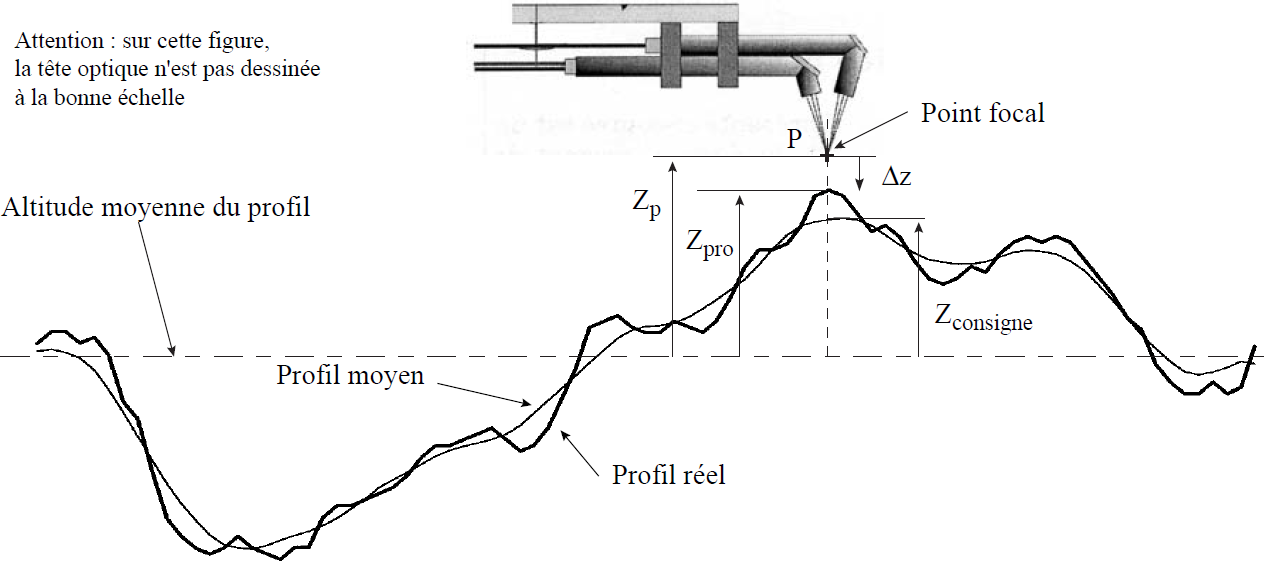
\includegraphics[width=.9\linewidth]{fig_08.png}
\caption{Simulation du stationnement \label{fig_08}}
\end{figure}

%Q8
\question{Quelles sont les exigences dimensionnelles vérifiées par la simulation (\autoref{fig_08}) et permettant de valider
la trajectoire ? Justifier les réponses apportées.}
\ifprof
\begin{corrige}
\end{corrige}
\else
\fi

La simulation a permis de valider la trajectoire à suivre. Cependant il faut encore établir le lien entre l’orientation
des roues directrices du véhicule et la trajectoire à suivre puisque le système de stationnement automatique agit
directement sur les roues directrices du véhicule.

\subsection{Direction du véhicule}

\begin{obj}
L’objectif est de déterminer la consigne angulaire des roues directrices du véhicule et sa vitesse de
recul lors de la phase d’insertion dans la place de stationnement.
\end{obj}


Pour l’étude il est choisi de prendre un véhicule type traction (roues avant motrices) comme 90\% des véhicules
vendus en France. De plus, la détermination de l’angle d’orientation des roues directrices (noté $\alpha$ sur la \autoref{fig_09})
sera limitée à la première portion de cercle $C_1$ pour laquelle le véhicule est en rotation autour du point $O_1$. Du
fait de la symétrie de la trajectoire, il n’est donc pas nécessaire de prolonger la détermination de $\alpha$ à la portion
de cercle $C_2$.

L’insertion du véhicule dans la place de stationnement peut se décomposer en trois phases à partir de l’instant
$t_0$ où le véhicule est à l’arrêt après avoir longé la place de stationnement envisagée.

\begin{itemize}
\item Phase 0 : recul rectiligne permettant au point $F$ d’atteindre le point $O$. La durée de cette phase est notée $\Delta T_0$.
\item Phase 1 : recul avec braquage des roues directrices, l’objectif étant que le point $F$ parcoure la portion de
cercle $C_1$ jusqu’au point $P$. La durée de cette phase est notée $\Delta T_1$.
\item Phase 2 : recul avec contre-braquage des roues directrices, l’objectif étant que le point $F$ parcoure la portion
de cercle $C_2$ jusqu’au moment où le véhicule est dans l’alignement de la place de stationnement. Comme la
manœuvre de stationnement se fait à vitesse constante et que les portions de cercle $C_1$
et $C_2$ sont symétriques, alors la durée de cette phase vaut également $\Delta T_1$.
\end{itemize}
Lors des phases de stationnement et entre chaque changement d’orientation des roues directrices du véhicule,
le véhicule recule à une vitesse supposée constante $v$ telle que $\vectv{C}{V}{\rep{1}}=v\vect{x_r}$. Dans la notation
$\vectv{C}{V}{\rep{1}}=v\vect{x_r}$. 
Dans la notation $\vectv{C}{V}{\rep{1}}=v\vect{x_r}$ $V$ désigne le véhicule et $\rep{1}\repere{O_1}{x_0}{y_0}{z_0}$
le repère galiléen défini au point $O_1$.

Le paramètre angulaire $\theta_1 = \angl{x_0}{y_0}$ (\autoref{fig_07}) définit la position relative de la base $\base{x_v}{y_v}{z_v}$
par rapport à la base $\base{x_0}{y_0}{z_0}$. Ainsi $\vecto{V}{\rep{1}} = \dot{\theta_1}\vect{z_0}$.

La \autoref{fig_09} représente le véhicule lors de la phase 1 de la manœuvre de stationnement. Comme l’orientation des
roues directrices (roues avant) sont liées entre elles, il n’est pas nécessaire de prendre en compte les deux roues.
$\alpha$ désigne l’angle que fait la roue intérieure au virage (côté trottoir) par rapport au véhicule (\autoref{fig_09}).

 $\alpha = \angl{x_v}{x_r}=\angl{y_v}{y_r}$
 avec $\rep{r} \repere{C}{x_r}{y_r}{z_r}$ 
un repère orthonormé direct défini au point $C$, centre de la roue intérieure, et tel que $\axe{C}{y_r}$ est confondu avec l’axe de cette roue (\autoref{fig_09}) et $\rep{v}\repere{F}{x_v}{y_v}{z_v}$ un repère
orthonormé défini au point $F$ et lié au véhicule (\autoref{fig_09}).


\begin{figure}[H]
\centering
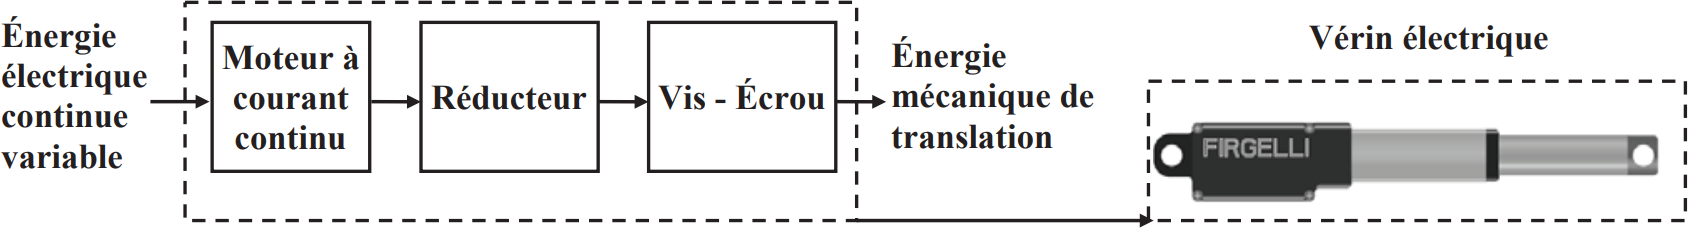
\includegraphics[width=.45\linewidth]{fig_09.png}
\caption{Paramétrage lors de la manoeuvre \label{fig_09}}
\end{figure}

Données : $\vect{FO_1}=R\vect{y_v}$, $\vect{CF}=L_t\vect{x_v}-e_t\vect{y_v}$ où $C$ est le centre de rotation de la roue intérieure avant par rapport au véhicule.

%Q9
\question{Déterminer en projection dans la base $\base{x_v}{y_v}{z_v}$ l'expression de $\vectv{C}{V}{\rep{1}}$ en fonction de $R$ $e_t$, $L_t$, $\dot{\theta_1}$.}
\ifprof
\begin{corrige}
\end{corrige}
\else
\fi

%Q10
\question{On rappelle que $\vectv{C}{V}{\rep{1}} = v \vect{x_r}$. À partir du résultat de la question précédente, déterminer, en fonction de $R$, $e_t$ et $L_t$, l'expression de $\tan\alpha$ des roues directrices lors de la phase 1 de la manœuvre. Cet angle noté $\alpha_{c1}$ est constant puisque le point $F$ parcourt $C_1$. $\alpha_{c1}$ représente la consigne angulaire à imposer aux roues directrices
lors de la phase 1.}
\ifprof
\begin{corrige}
\end{corrige}
\else
\fi

Lors de la manœuvre de stationnement, l’angle des roues devra suivre une consigne de position angulaire notée $\alpha_c(t)$ à définir pour respecter les trois phases de l’insertion dans la place.

%Q 11. 
\question{Sous forme d’un graphique, proposer l’évolution temporelle de la consigne $\alpha_c(t)$ pour que le véhicule puisse s’insérer dans la place de stationnement selon les trois phases de manœuvre définies précédemment.
Sur ce graphique devront apparaitre les ordonnées particulières que $\alpha$ devra atteindre ainsi que les durées des
différentes phases de la manœuvre en fonction des données littérales du texte.}
\ifprof
\begin{corrige}
\end{corrige}
\else
\fi


Dans cette deuxième partie il a été possible de définir la trajectoire du véhicule et la consigne angulaire d’orientation des roues afin que le véhicule puisse effectuer la manœuvre en créneau en une fois. Ceci étant, le suivi de la trajectoire dépend des performances du système d’orientation des roues directrices. Ce système appelé
« direction » en automobile a son comportement défini par l’algorithme de stationnement lors de manœuvres
automatiques. Il est donc nécessaire de vérifier que la commande en direction permet effectivement de suivre la
trajectoire.

\textit{Pour la suite du sujet le support technique utilisé est une voiture radio commandée comme expliqué en début de sujet.}

\section{Modélisation de la commande de direction et validation des performances}
Le choix d’une voiture radio commandée (voiture RC) est motivé par la nécessité d’identifier les composants (et
leurs caractéristiques) intervenant dans la commande de direction, mais également par la nécessité de pouvoir
analyser des résultats d’essais réalisés sur un support réel. Tout ceci n’est pas possible sur un véhicule réel du
fait de la confidentialité des données des constructeurs automobiles, mais concernant un modèle réduit il n’y a
plus ces difficultés.

La \autoref{fig_10} représente le modèle de voiture RC choisi pour la suite de l’étude.

\begin{figure}[H]
\centering
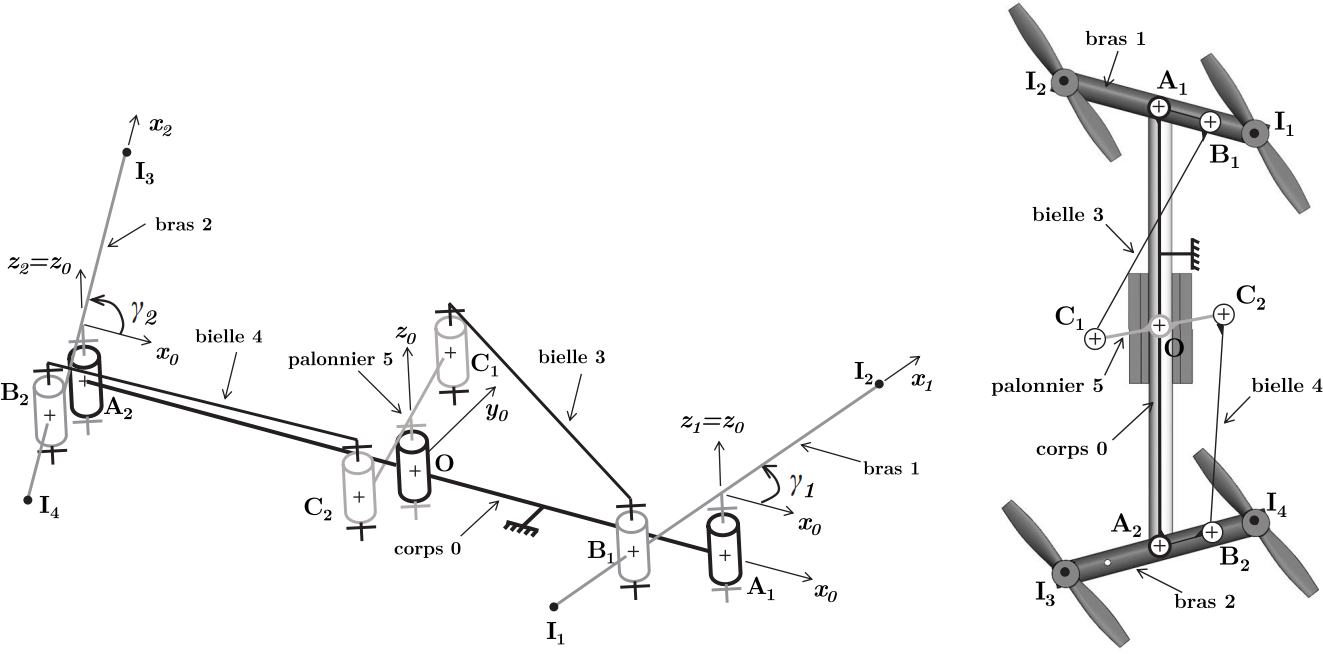
\includegraphics[width=.45\linewidth]{fig_10.png}
\caption{Tamiya M-05 Mazda \label{fig_10}}
\end{figure}

Le choix de la voiture radio commandée est pertinent pour les raisons suivantes :
\begin{itemize}
\item les résultats obtenus en première partie de sujet sont transposables à plus petite échelle ;
\item la voiture RC possède des proportions identiques à un véhicule réel (échelle un dixième) et est de type
traction comme dans la première partie ;
\item compte tenu de la faible vitesse de déplacement du véhicule, les effets dynamiques dûs au déplacement du
véhicule ne seront pris en compte dans les études suivantes ;
\item à part l’actionneur, la structure de la direction est assimilable à celle des véhicules réels.
\end{itemize}

\begin{obj}
La trajectoire d’insertion dans une place de stationnement est certes déterminée, mais il reste à évaluer
la capacité du véhicule à suivre cette trajectoire. L’objectif de cette partie est donc de synthétiser la
commande du système de direction du véhicule choisi permettant à ce dernier d’exécuter la manœuvre
d’insertion en créneau telle que définie en première partie de sujet.
\end{obj}

\subsection{Modélisation de la direction du véhicule radio commandé}

L’objectif est d’établir le modèle de la commande de direction du véhicule RC à implanter dans l’algorithme
de stationnement afin de pouvoir déterminer les performances de cette commande et d’évaluer la nécessité ou
non d’optimiser cette dernière. L’algorithme d’assistance au stationnement pilotant la direction du véhicule,
cette dernière doit avoir des performances garantissant le suivi de la trajectoire calculée pour la manœuvre de
stationnement.
Les performances attendues pour cette commande sont recensées dans le \autoref{tab_02}.

\begin{table}[H]
\centering
\begin{tabular}{lll}
\hline
Performance &Critère& Niveau \\
\hline 
Précision angulaire & Erreur &Nulle en régime permanent pour une entrée en échelon \\
Rapidité &Temps de réponse à 5\% & $t_{r5\%}\leq \SI{0,4}{s}$ \\
Stabilité &Dépassement &Aucun \\ \hline
\end{tabular}
\caption{Performances attendues de l’asservissement en position des roues directrices du véhicule RC
 \label{tab_02}}
\end{table}

\subsubsection{Étude structurelle de la direction du véhicule radio commandé}
\question{À partir des documents relatifs à la direction du véhicule RC fournis \autoref{fig_27} à \autoref{fig_29} 
identifier à quoi correspondent les numéros figurant sur la description chaine d’énergie / chaine d’information
\autoref{fig_11}.}
\ifprof
\begin{corrige}
\end{corrige}
\else
\fi

\begin{figure}[H]
\centering
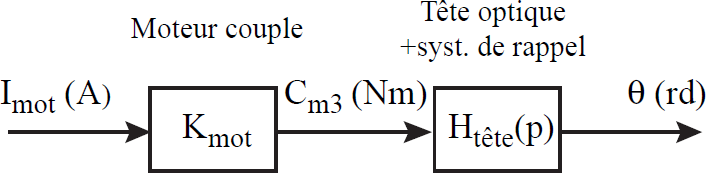
\includegraphics[width=\linewidth]{fig_11.png}
\caption{Description chaine d’énergie / chaine d’information de la direction \label{fig_11}}
\end{figure}

\subsubsection{Commande angulaire des roues directrices}
La commande angulaire des roues directrices est fournie \autoref{fig_12}. Cette commande permet d’imposer l’angle des roues directrices $\alpha(t)$ (\autoref{fig_09}) en fonction d’un angle de consigne $\alpha_c(t)$ (dont l’évolution a été caractérisée en fin de seconde partie).


\begin{figure}[H]
\centering
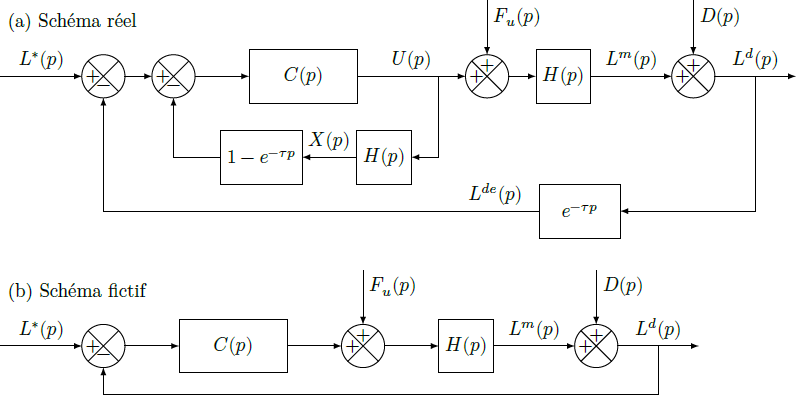
\includegraphics[width=\linewidth]{fig_12.png}
\caption{Schéma blocs de la commande en position des roues directrices du véhicule RC \label{fig_12}}
\end{figure}

\textbf{Données et notations}
\begin{itemize}
\item $A_{c}(p)$, $A_{1c}(p)$, $A_{1}(p)$, $U_m(p)$, $U_{\text{mes}}(p)$, $U_c(p)$, $\Omega_m(p)$ et 
$\Omega_1(p)$ sont respectivement les transformées de Laplace des grandeurs 
$\alpha_{c}(t)$, $\alpha_{1c}(t)$, $\alpha_{1}(t)$, $u_m(t)$, $u_{\text{mes}}(t)$, $u_c(t)$, $\omega_m(t)$ et $\omega_1(t)$.
\item Les conditions initiales sont supposées nulles.
\item $K_c = \SI{1,05}{V.rad^{-1}}$ et $K_r=1/120$.
\item À ce stade de l’étude la commande est étudiée sans correction $C(p)=1$.
\end{itemize}
Pour cette première étude de la commande de direction, le véhicule est maintenu horizontal mais n’est pas en
contact avec le sol.

La boucle d’asservissement est réalisée sur le servomoteur. L’angle de consigne $\alpha_{c}(t)$ est converti en angle de
consigne $\alpha_{1c}(t)$ pour le servomoteur. Le bloc $H_t(p)$ modélise dans le domaine de Laplace la relation entre $\alpha(t)$ et $\alpha_1(t)$ l’angle de rotation en sortie du servomoteur. Ainsi le bloc $H_t(p)$ correspond à la modélisation de la transmission de mouvement dans la direction (ensemble des bielles et des bras composant la direction du véhicule).

Le gain $K_a$ est un gain d’adaptation permettant de convertir l’angle de consigne $\alpha_{1c}(t)$ (en radians) en une tension de consigne $u_{c}(t)$ (en volts). La tension $u_{\text{mes}}(t)$ est l’image en volts de l’angle $\alpha_1(t)$ (en radians) du bras
1 du servomoteur. Le gain $K_c$ 
(en \si{V.rad^{-1}}) modélise le potentiomètre équipant le servomoteur.
La tension de commande $u_{m}(t)$ du servomoteur est directement générée à partir de $u_{c}(t) -u_{\text{mes}}(t)$ par un
correcteur de fonction de transfert $C(p)$. Le moteur du servomoteur est modélisé par le bloc $H_m(p)$. Le taux de rotation du moteur est noté $\omega_m(t)$. Le gain $K_r$ correspond au rapport de réduction du réducteur du servomoteur.

Le bras \textbf{1} du servomoteur est monté sur l’axe de sortie du réducteur du servomoteur. $\omega_1(t)$ est le taux de rotation (en \si{rad.s^{-1}} du bras du servomoteur.
Afin d’établir le modèle de la commande angulaire de la direction non corrigée et d’en déterminer les performances, il est nécessaire d’identifier les modèles et les caractéristiques des différents composants.

\paragraph{Modélisation de la transmission de la direction et détermination de $H_t(p)$}

\begin{obj}
L’objectif est de déterminer l’expression de $H_t(p)=\dfrac{A(p)}{A_1(p)}$ 
modélisant la transmission mécanique entre le bras \textbf{1} du servomoteur et la roue \textbf{6}.
\end{obj}

La \autoref{fig_13} représente le schéma cinématique de la direction dans le plan $\left(A,\vect{x},\vect{y}\right)$ avec $\rep{}\repere{A}{x}{y}{z}$ un repère
galiléen dont le vecteur $\vect{z}$ est vertical ascendant. La direction est sans jeu et les liaisons sont supposées parfaites.

\begin{figure}[H]
\centering
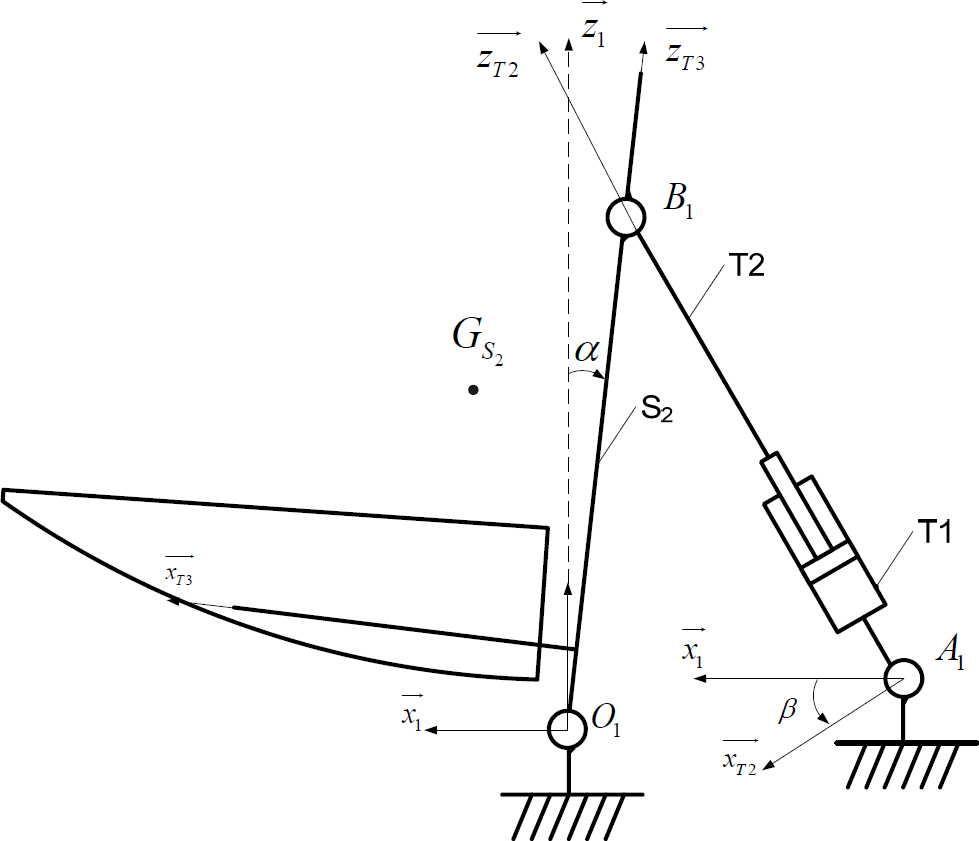
\includegraphics[width=.6\linewidth]{fig_13.png}
\caption{Schéma cinématique plan de la direction du véhicule radio commandé \label{fig_13}}
\end{figure}


$\rep{1}\repere{A}{x_1}{y_1}{z}$  est un repère orthonormé lié au bras \textbf{1},
$\rep{6}\repere{P}{x_6}{y_6}{z}$  est un repère orthonormé lié à l’ensemble \textbf{6} \{fusée + roue\}.
 Ainsi $\alpha_1 = \angle{x}{x_1}$ et $\alpha = \angle{x}{x_6}$.

Le bâti \textbf{0} représente le châssis du véhicule RC. Les deux roues sont orientées grâce à un seul actionneur.
Afin de déterminer l’expression de $\alpha(t)$ en fonction de $\alpha_1(t)$, il est nécessaire d’étudier deux chaines fermées de
solides et de liaisons : la chaine \{0, 1, 2, 3, 0\} et la chaine \{0, 3, 4, 6, 0\}.
La \autoref{fig_14} présente le paramétrage lié aux solides 1, 2 et 3.

\textbf{Paramétrage}
\begin{itemize}
\item $\rep{2}\repere{B}{x_2}{y_2}{z}$ est un repère orthonormé lié à la tige \textbf{2} et 
$\rep{3}\repere{D}{x_3}{y_3}{z}$ un repère orthonormé lié à la
bielle de renvoi \textbf{3}.
\item $\vect{AB}=\ell_1\vect{x_1}$, $\vect{BC}=b\vect{x_2}$, $\vect{CD}=\left(a-\ell_1\right)\vect{x_3}$, $\vect{AD}=a\vect{x}+b\vect{y}$ et $\vect{DE}=\ell_3\vect{y_3}$.
\item $\alpha_1=\angl{x}{x_1}$, $\alpha_2=\angl{x}{x_2}$, $\alpha_3=\angl{x}{x_3}$.
\end{itemize}

%Q13
\question{En exploitant la fermeture géométrique de la chaine \{0, 1, 2, 3, 0\} et en faisant l’hypothèse que l’angle $\alpha_2$ varie très peu $\alpha_2\simeq 90\degres$, montrer que $\sin\alpha_3 = k\sin\alpha_1$ et préciser l’expression de $k$.}
\ifprof
\begin{corrige}
\end{corrige}
\else
\fi

La \autoref{fig_15} représente l’évolution de $\alpha_3$  en fonction de $\alpha_1$ pour un seul des deux sens de rotation des roues ($\alpha_3$ varie de $0\degres$ à $-45\degres$). Lorsque les roues sont parallèles au véhicule $\alpha_1 = 0\degres$ et $\alpha_3 = 0\degres$.

%Q14
\question{À partir de la \autoref{fig_15} justifier que $\alpha_3 = K_{31}\alpha_1$
en précisant la valeur de la constante $K_{31}$.
En raisonnant de façon similaire, l’étude de la chaine fermée \{0, 3, 4, 6, 0\} permet de montrer que $\alpha$ est
proportionnel à $\alpha_3$.}
\ifprof
\begin{corrige}
\end{corrige}
\else
\fi

Ainsi, pour la suite de l’étude il est considéré que $\alpha=\lambda\alpha_1$, avec $\lambda$ une constante supposée connue. Ainsi pour la suite de l’étude $H_t(p)=\lambda$.



\begin{figure}[H]
\centering
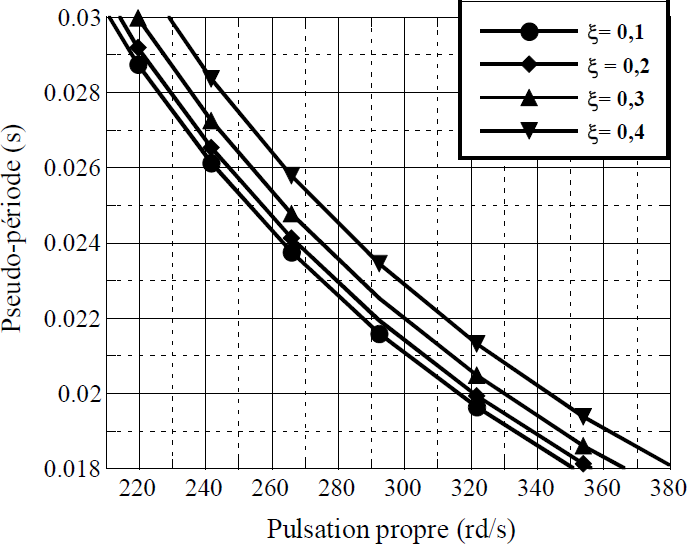
\includegraphics[width=.45\linewidth]{fig_14.png}
\caption{Schéma cinématique plan de la direction du véhicule radio commandé \label{fig_14}}
\end{figure}


\begin{figure}[H]
\centering
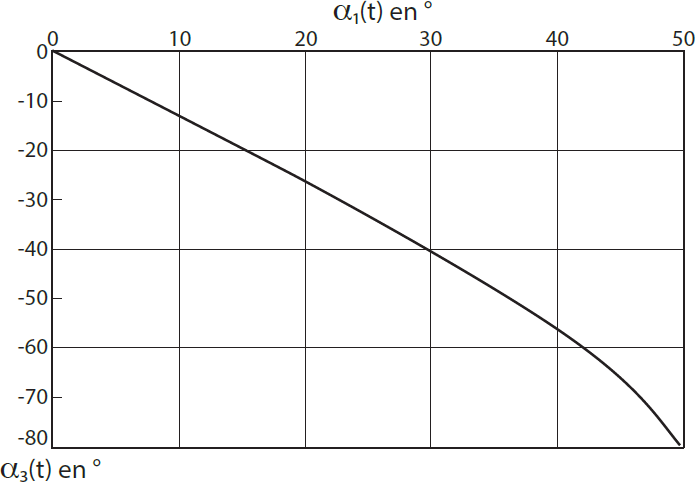
\includegraphics[width=.45\linewidth]{fig_15.png}
\caption{Tracé de $\alpha_3(t)$ en fonction de $\alpha_1(t)$ \label{fig_15}}
\end{figure}

Toujours dans l’objectif de modéliser la commande de la direction il est nécessaire de s’intéresser à son comportement dynamique.

\paragraph{Comportement dynamique de la direction et modélisation du servomoteur}

\begin{obj}
L’objectif est d’écrire l’équation comportementale de la direction permettant d’identifier le bloc $H_m(p)$.
\end{obj}

L’axe du moteur du servomoteur, dont le taux de rotation par rapport au châssis est noté $\omega_m(t)$, est soumis à un couple moteur défini pa
$\torseurstat{T}{\text{moteur}}{1} =\torseurl{\vect{0}}{C_m\vect{z}}{A}$. 

Le couple dû aux frottements visqueux présents dans la direction est modélisé par une action mécanique extérieure appliquée au bras 1 : $\torseurstat{T}{\text{ext}}{1} = \torseurl{\vect{0}}{-f\dot{\alpha}_1(t) \vect{z}}{A}$ avec $g = 8,87 \times 10^{-8} \si{Nms}$  le coefficient de viscosité.
Pour cette étude le véhicule est à l’horizontale mais n’est pas en contact avec le sol. Une étude du comportement
dynamique de la direction permet d’obtenir 
$J_{\text{eq}}\dfrac{\dd\dot{\alpha}_1(t)}{\dd t} = C_m(t)-f\dot{\alpha_1}(t)$.

Cette équation a été obtenue à partir du théorème de l’énergie cinétique appliqué à l’ensemble 
$\Sigma =$\{réducteur et axe moteur du servomoteur,1, 2, 3, 3’, 4, 4’, 5, 6, 6’\} en mouvement par rapport au châssis du véhicule supposé galiléen.



\textbf{Données et notations}
\begin{itemize}
\item Les solides 1, 2, 3, 3’, 4 et 4’ sont supposés de masse négligeable par rapport à la masse des autres solides
de la direction.
\item $J_m$ (inconnu) est le moment d’inertie équivalent de l’ensemble {axe moteur + réducteur} du servomoteur rapporté à l’axe $\axe{A}{z}$ de sortie du servomoteur.
\item Le solide 5 est en mouvement de translation et sa masse est notée $m_5$.
\item $J_6$ est le moment d’inertie de l’ensemble 6 selon l’axe $\axe{P}{z}$.
\item $J'_6$ est le moment d’inertie de l’ensemble 6’ selon l’axe $\axe{P'}{z'}$ et $J_6 = J_6'$.
\item $J_{\text{eq}}$ représente le moment d’inertie équivalent de tous les solides en mouvement lors de l’orientation des roues et rapporté à l’axe $\axe{A}{z}$ de sortie du servomoteur.
\item Le rapport de réduction du réducteur du servomoteur est $K_r = \dfrac{1}{120}$.
\item On considère que l’angle de direction $\alpha = \axe{x}{x_6}$ est égal pour les roues directrices (\autoref{fig_13}). C’est le cas
sur le modèle RC puisque l’ensemble \{3, 3’, 5\} forme un parallélogramme déformable.
\end{itemize}

%Q15
\question{Faire un inventaire des puissances des actions mécaniques extérieures et intérieures mises en jeu dans le théorème de l’énergie cinétique appliqué à $\Sigma$ fournissant l’équation différentielle précédente. Une attention particulière sera portée à la classification, au caractère lisible, compréhensible et justifié de l’inventaire. L’expression des puissances des actions mécaniques extérieures et intérieures est exigée.}
\ifprof
\begin{corrige}
\end{corrige}
\else
\fi

%Q16
\question{Déterminer l’expression de $\vectv{E}{3}{0}$ et de $\vectv{E}{5}{0}$ en fonction de $\dot{\alpha_1}(t)$.}
\ifprof
\begin{corrige}
\end{corrige}
\else
\fi

%Q 17. 
\question{Déterminer l’expression des énergies cinétiques $\ec{S}{0}$ ($S$ désignant l’ensemble \{axe moteur + réducteur\} du servomoteur), $\ec{5}{0}$, $\ec{6}{0}$ et $\ec{6'}{0}$ en fonction de $\alphap(t)$.}
\ifprof
\begin{corrige}
\end{corrige}
\else
\fi

%Q 18. 
\question{Écrire l’expression de l’énergie cinétique $\ec{\Sigma}{0}$ en fonction de $\alphap(t)$ et en déduire l’expression de l’inertie équivalente $\indice{J}{eq}$.}
\ifprof
\begin{corrige}
\end{corrige}
\else
\fi

Pour finaliser la modélisation de la commande, il est nécessaire d’identifier toutes les caractéristiques du servomoteur dont $J_m$.

\paragraph{Identification du servomoteur}

Pour déterminer les caractéristiques du servomoteur, on procède à des mesures sur celui-ci, lorsqu’il n’est pas
en liaison avec le reste de la direction. La figure 16 représente une modélisation sous forme de schéma-blocs du
servomoteur.


\begin{figure}[H]
\centering
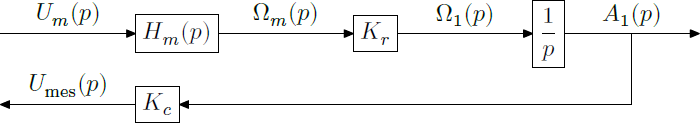
\includegraphics[width=.55\linewidth]{fig_16.png}
\caption{Schéma-blocs du servomoteur seul \label{fig_16}}
\end{figure}

Les équations disponibles pour la modélisation du fonctionnement du servomoteur sont :
\begin{itemize}
\item en notant $R$ la résistance aux bornes de l’induit, $L$ l’inductance aux bornes de l’induit, $i(t)$ l’intensité moteur et $e(t)$ la force contre-électromotrice, $L\dfrac{\dd i(t)}{\dd t} +Ri(t) =u_m(t)-e(t)$;
\item avec $k_e$ la constante de vitesse du moteur en \si{V.s.rad^{-1}} et $\omega_m(t)$ le taux de rotation du moteur du servomoteur par rapport au châssis de la voiture, $e(t)=k_e\omega_m(t)$;
\item avec $C_m(t)$ le couple moteur, $k_t$ la constante de couple en \si{N.m.A^{-1}} et $k_t=k_e$, 
$C_m(t)=k_t i(t)$;
\item en négligeant les autres actions mécaniques mises en jeu dans la direction par rapport au couple moteur
$C_m(t)$, $J_m\dfrac{\dd \omega_1(t)}{\dd t} = C_m(t)$;
\item enfin $\omega_1=\dfrac{\dd \alpha_1(t)}{\dd t}$.
\end{itemize}

Aucune donnée n’est accessible pour le moteur à courant continu utilisé ainsi que pour le servomoteur à part
$K_r$ donné précédemment. Une série d’essais en boucle ouverte est réalisée afin de déterminer les caractéristiques $R$, $L$ et $J_m$ du servomoteur.
La \autoref{fig_17} représente l’évolution de la tension $\indice{u}{mes}(t)$ fournie par le potentiomètre du servomoteur pour un échelon de tension $u_m(t) = u_0 = \SI{3}{V}$ en boucle ouverte.

\begin{figure}[H]
\centering
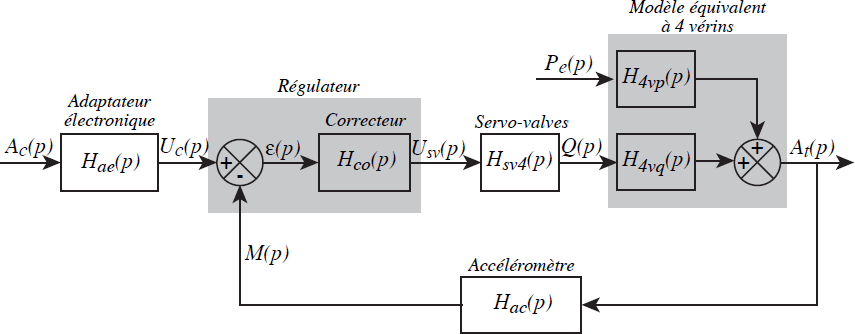
\includegraphics[width=.45\linewidth]{fig_17.png}
\caption{Tension fournie par le potentiomètre du servomoteur pour un échelon de tension $u_m(t)=\SI{3}{V}$ \label{fig_17}}
\end{figure}

L’expression temporelle de $\indice{u}{mes}(t)$ correspondant au comportement observé \autoref{fig_17} est
$\indice{u}{mes}(t) = K_m K_c K_r u_0\left(t-\tau_m\right)+K_m K_c K_r\tau_m u_0 \text{e}^{-\dfrac{t}{\tau_m}}$.

Il est possible de mettre $H_m(p)$ sous la forme $H_m(p) = \ordreunopt{K_m}{\tau_m}$
avec $K_m = \dfrac{1}{k_e}$ et $\tau_m =\dfrac{R J_m}{k_e^2}$.

\question{À partir de l’expression temporelle de $\indice{u}{mes}(t)$ donnée précédemment, déduire de l’essai \autoref{fig_17} les valeurs numériques des constantes $K_m$ et $\tau_m$. Il est rappelé que $K_c = \SI{1,05}{V.rad^{-1}}$.}
\ifprof
\begin{corrige}
\end{corrige}
\else
\fi

%Q20
\question{Déduire la valeur numérique de $k_e$ et de $RJ_m$.}
\ifprof
\begin{corrige}
\end{corrige}
\else
\fi

La \autoref{fig_18} représente l’évolution de l’intensité moteur pour un échelon de tension $u_m(t)=\SI{3}{V}$ avec le rotor du moteur bloqué.

\begin{figure}[H]
\centering
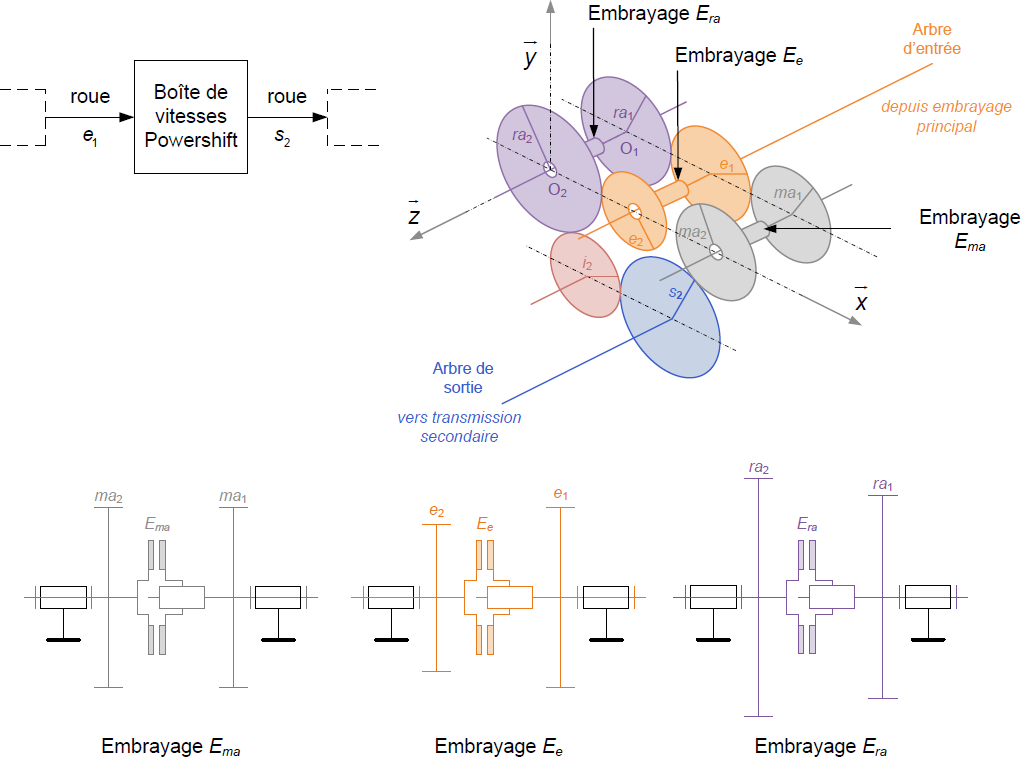
\includegraphics[width=.45\linewidth]{fig_18.png}
\caption{Intensité moteur\label{fig_18}}
\end{figure}

%Q21
\question{Exprimer la fonction de transfert $\dfrac{I(p)}{U_m(p)}$ sous forme canonique lorsque le rotor est bloqué.}
\ifprof
\begin{corrige}
\end{corrige}
\else
\fi

%Q22
\question{Déduire de la \autoref{fig_18} la valeur numérique de $R$ et celle de $L$. À partir des résultats obtenus par l’exploitation de la \autoref{fig_17}, déduire également la valeur numérique de $J_m$.}
\ifprof
\begin{corrige}
\end{corrige}
\else
\fi

$J_m$étant identifié, avec la connaissance des moments d’inertie des solides constituant la direction il est possible
d’en déduire l’inertie équivalente $J_{\text{eq}}$.

Au vu des vitesses de déplacement des solides composant la direction, les actions mécaniques dues au frottement
visqueux sont très petites vis-à-vis des autres actions mécaniques mises en jeu. Ainsi pour le modèle de l’ensemble
de la commande en position des roues directrices $H_m(p) = \ordreunopt{K_m}{\tau_m}$ avec $K_m$ et $\tau_m = \dfrac{RJ_{\text{eq}}}{k_e^2}$ identifiés.
À ce stade de l’étude, il reste à déterminer la fonction de transfert de la commande asservie d’orientation des
roues. Cette dernière ne faisant pas encore intervenir de correction et il va être nécessaire de caractériser les
performances de la commande afin d’identifier le besoin ou non d’une correction.

\subsubsection{Modèle global et performances de la commande sans correction}
\begin{obj}
L’objectif de cette section est d’analyser les performances, caractérisées dans le \autoref{tab_02}, de
la commande de direction sans correction : $C(p)=1$.
\end{obj}
Pour la suite $K_m =\SI{256}{rad.s^{-1}V^{-1}}$ et $\tau_m = \SI{0,03}{s}$ et il est rappelé que $K_c = \SI{1,05}{V.rad^{-1}}$ et $K_r = 1/120$.

%Q23
\question{Afin que l’asservissement soit de qualité il est nécessaire que l’écart $\varepsilon(t)$ soit nul quand $\alpha(t)=\alpha_c(t)$ en régime permanent et pour une entrée type échelon. Déterminer la relation entre $K_a$ et $K_c$ permettant un asservissement de qualité.}
\ifprof
\begin{corrige}
\end{corrige}
\else
\fi

Les différentes fonctions de transfert du modèle \autoref{fig_12} étant identifiées, il est maintenant possible d’établir la fonction de transfert $H(p)=\dfrac{A(p)}{A_c(p)}$.

%Q 24. 
\question{Déterminer l’expression de $H(p)$, fonction de transfert de la commande des roues. Mettre $H(p)$ sous
forme canonique, préciser l’ordre de $H(p)$ et l’expression de ses paramètres caractéristiques. Faire les applications numériques.}
\ifprof
\begin{corrige}
\end{corrige}
\else
\fi

%Q 25. 
\question{À partir des résultats de la question précédente et en se référant au \autoref{tab_02}, conclure sur
les performances de précision angulaire et d’amortissement du modèle théorique de la commande des roues.}
\ifprof
\begin{corrige}
\end{corrige}
\else
\fi

La figure 19 montre, pour une entrée en échelon  $\alpha_c(t)$ d’amplitude $\pi/4 \si{rad}$ :
\begin{itemize}
\item l’évolution de l’angle $\alpha(t)$ obtenue avec le modèle théorique établi précédemment ;
\item la courbe expérimentale de $\alpha(t)$ obtenue pour un essai réalisé avec la voiture RC à l’horizontale et sans contact avec le sol.
\end{itemize}

\begin{figure}[H]
\centering
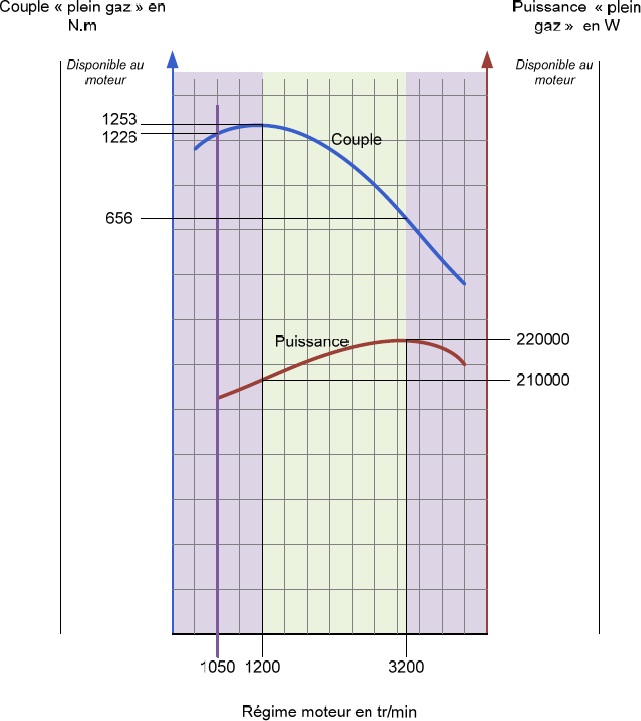
\includegraphics[width=.45\linewidth]{fig_19.png}
\caption{Acquisition de l’orientation des roues directrices \label{fig_19}}
\end{figure}

%Q 26. 
\question{Conclure sur la validité du modèle théorique de la commande des roues vis-à-vis du comportement
réel observable \autoref{fig_19}. Qu’il s’agisse du modèle théorique ou du comportement réel de la commande des roues,
conclure sur la performance en rapidité.}
\ifprof
\begin{corrige}
\end{corrige}
\else
\fi

Un modèle théorique de la commande des roues ayant été établi, il va permettre de synthétiser une correction
pour l’asservissement en position des roues afin d’en améliorer les performances qui ne sont pas encore respectées

\section{Amélioration des performances  -- choix d’une correction de la
commande}
\begin{obj}
L’objectif de cette partie est de choisir un correcteur à implanter dans la commande afin que cette
dernière vérifie tous les critères de performance assurant le suivi de la trajectoire désirée (\autoref{tab_02})
\end{obj}

Pour cette partie le schéma blocs de la commande des roues (véhicule hors sol) est donné \autoref{fig_20} et $G(p) = \dfrac{K}{p\left(1+\tau p\right)}$  avec $K = \SI{2,2}{rad.V^{-1}.s^{-1}}$ et $\tau = \SI{0,015}{s}$.$K$ et $\tau$ sont fonction des paramètres de la commande définis dans la partie précédente.


\begin{figure}[H]
\centering
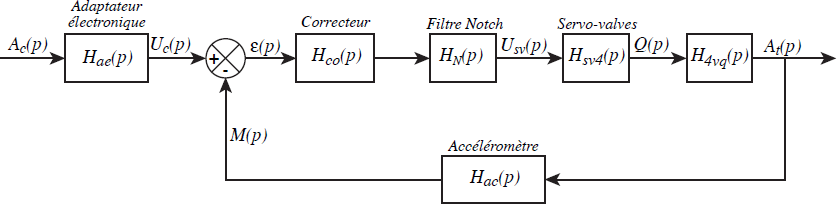
\includegraphics[width=.45\linewidth]{fig_20.png}
\caption{Schéma blocs de la commande en position des roues \label{fig_20}}
\end{figure}


\subsection{Amélioration et correction du modèle de l’asservissement en position des roues}
Il est décidé, dans un premier temps, d’utiliser une action proportionnelle $C(p)=K_P$ avec $K_P$ une constante
homogène à des \si{V.rad^{-1}}. L’objectif est donc de déterminer le paramètre $K_p$ afin d’améliorer la performance de rapidité du modèle théorique de la commande des roues.

%Q27
\question{Après avoir donné l’expression de $H(p) = \dfrac{A(p)}{A_c(p)}$, déterminer l’expression de $K_p$ pour que la commande soit la plus rapide possible sans dépassement pour une consigne de type échelon. Faire l’application numérique.}
\ifprof
\begin{corrige}
\end{corrige}
\else
\fi

La \autoref{fig_21} représente la réponse temporelle théorique $\alpha(t)$ de la commande des roues pour une consigne $\alpha_c(t)$ en échelon d’amplitude $\pi/4$ et pour la valeur de $K_p$ déterminée précédemment.


\begin{figure}[H]
\centering
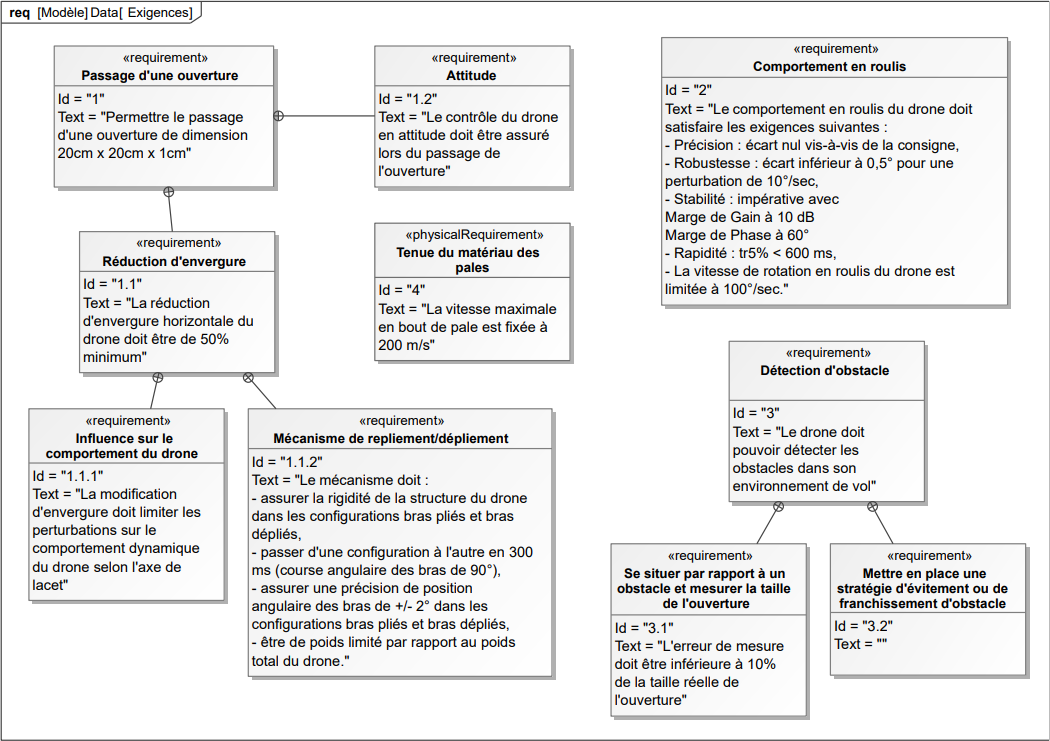
\includegraphics[width=.45\linewidth]{fig_21.png}
\caption{Évolution temporelle de $\alpha(t)$ pour une correction proportionnelle \label{fig_21}}
\end{figure}

%Q 28.
\question{À partir de la \autoref{fig_21}, conclure sur l’effet de la correction choisie vis-à-vis des performances attendues pour la commande des roues du véhicule RC.}
\ifprof
\begin{corrige}
\end{corrige}
\else
\fi

\subsection{Performances dans le domaine réel et amélioration de la correction}

\begin{obj}
L’objectif est de choisir et valider une forme définitive de correction à appliquer à la commande des
roues.
\end{obj}

La \autoref{fig_22} représente deux essais avec la direction du véhicule RC en utilisant la correction proportionnelle.
Un essai a été réalisé avec le véhicule ne touchant pas le sol et un second avec le véhicule posé sur le sol, dans
les deux cas le véhicule est à l’arrêt et la consigne $\alpha_c(t)$ en échelon d’amplitude $\pi/4$.

\begin{figure}[H]
\centering
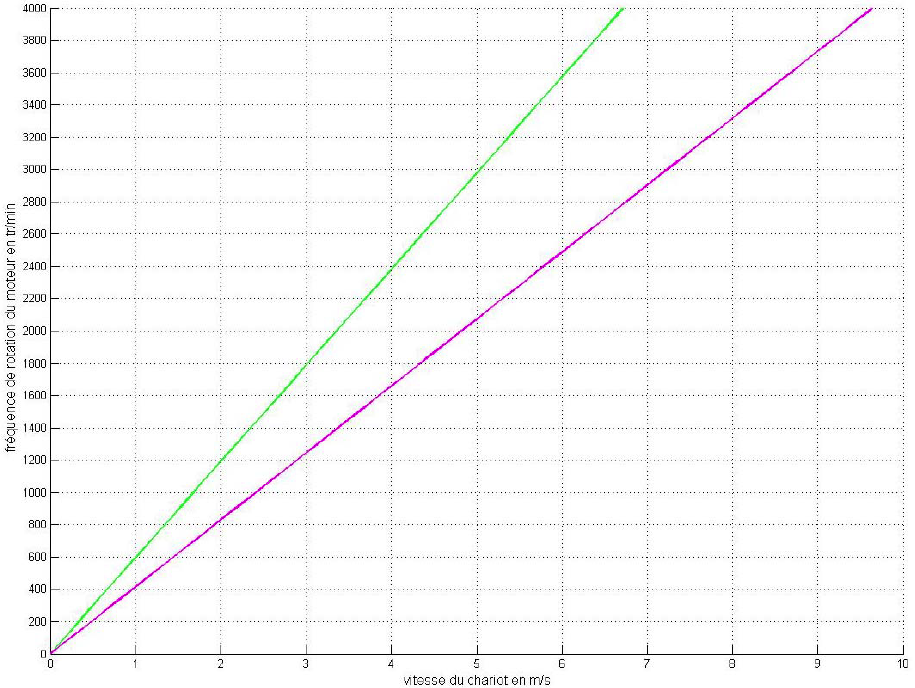
\includegraphics[width=.45\linewidth]{fig_22.png}
\caption{Essais expérimentaux réalisés sur le véhicule RC \label{fig_22}}
\end{figure}

\question{Conclure sur la performance en précision de la commande des roues en expliquant la cause possible
de l’écart observé entre les deux courbes expérimentales de la \autoref{fig_22}.}
\ifprof
\begin{corrige}
\end{corrige}
\else
\fi

Afin de rendre la direction insensible aux perturbations, une action de type intégrale en complément de l’action
proportionnelle est envisagée pour le correcteur. La \autoref{fig_23} représente les diagrammes de Bode en boucle ouverte de la commande théorique des roues directrices pour $C(p)=\dfrac{K_p}{p}$ 
(intégrateur) et $C(p)=K_p\left(1+\dfrac{1}{T_i p}\right)$ (proportionel intégral) avec $T_i = \SI{0,8}{s}$.

\begin{figure}[H]
\centering
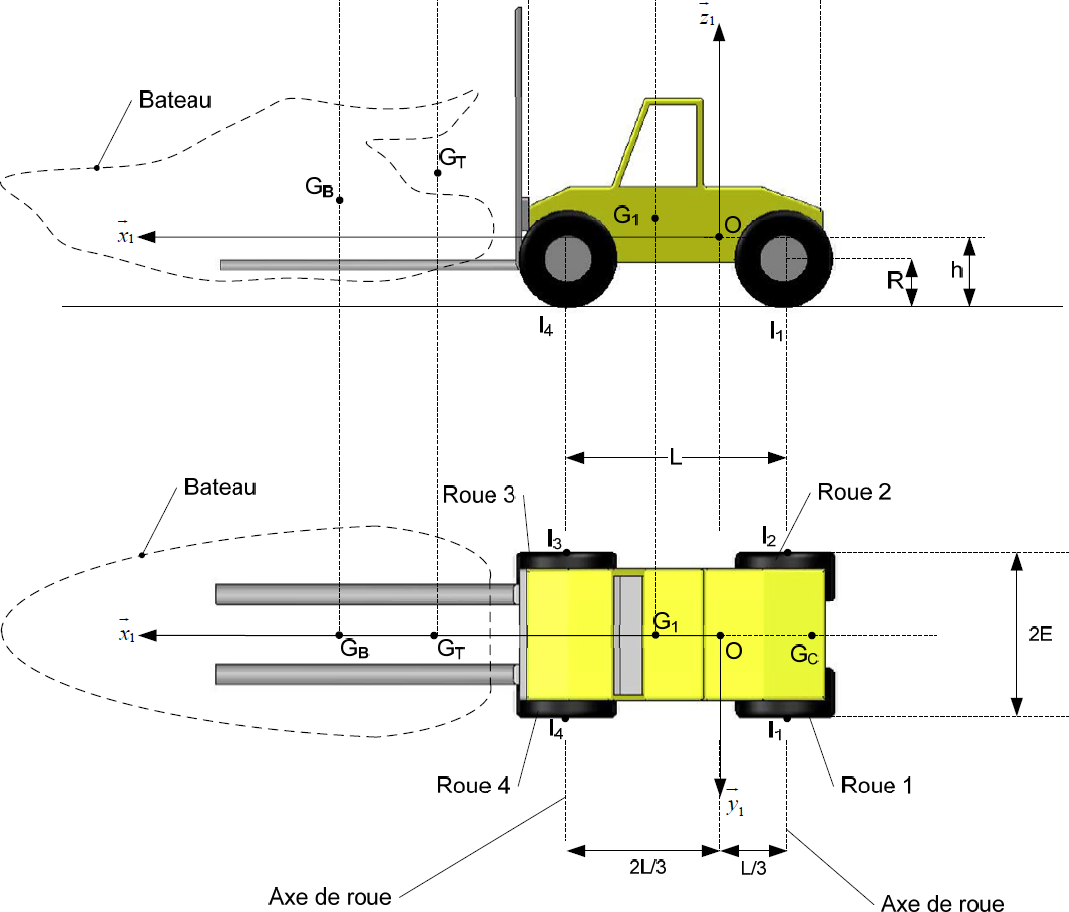
\includegraphics[width=.45\linewidth]{fig_23.png}
\caption{Diagrammes de Bode de la FTBO corrigée \label{fig_23}}
\end{figure}

%Q 30. 
\question{Quel correcteur choisir pour que le système soit stable ? Justifier la réponse.}
\ifprof
\begin{corrige}
\end{corrige}
\else
\fi

L’étude précédente a permis de caractériser un correcteur assurant à la commande des roues les performances
attendues et une robustesse vis-à-vis de perturbations. Le modèle de l’asservissement corrigé peut être implanté
dans l’algorithme pour le suivi de trajectoire de stationnement.


\section{Conclusion et synthèse}

La \autoref{fig_24} représente une mesure de l’angle $\alpha(t)$ des roues directrices avec le correcteur précédemment déterminé implanté dans la commande des roues. Cet essai a été effectué avec le véhicule RC posé au sol et à l’arrêt.

\begin{figure}[H]
\centering
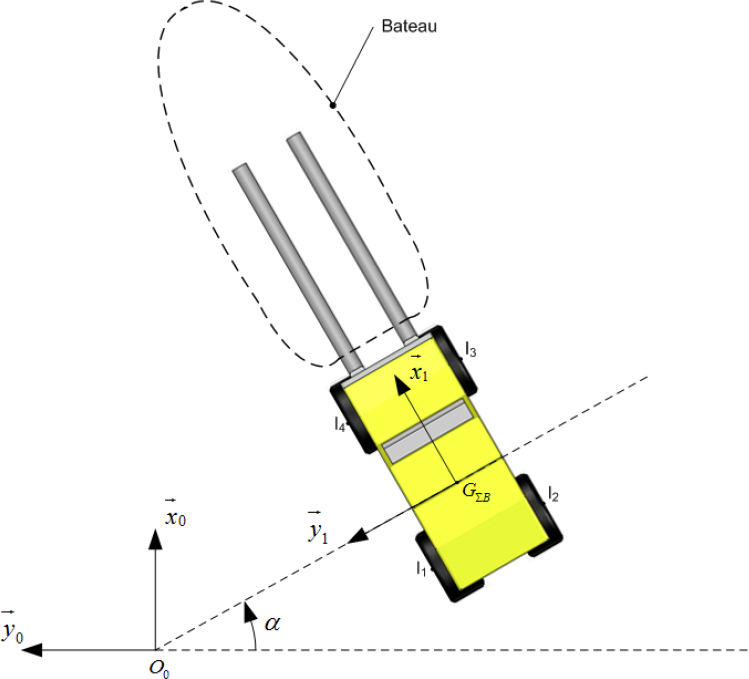
\includegraphics[width=.45\linewidth]{fig_24.png}
\caption{Angle des roues directrices \label{fig_24}}
\end{figure}

%Q 31
\question{À partir de la  \autoref{fig_24}, conclure sur le comportement de la commande des roues vis-à-vis des performances de précision, de stabilité et de rapidité attendues.}
\ifprof
\begin{corrige}
\end{corrige}
\else
\fi

Un essai d’insertion du véhicule RC dans une place libre a été réalisé permettant d’obtenir la  \autoref{fig_25}. Sur
cette figure sont représentés :
\begin{itemize}
\item l’angle de consigne des roues directrices $\alpha_c(t)$ ;
\item l’angle réel des roues directrices $\alpha(t)$;
\item la trajectoire théorique du point $F$ pour la consigne $\alpha_c(t)$, le véhicule se déplaçant à vitesse constante ;
\item la trajectoire réelle du point $F$.
\end{itemize}

%Q 32. 
\question{Expliquer la cause des écarts observés entre la trajectoire théorique et la trajectoire réelle.
Comme le montre la  \autoref{fig_25}, la manœuvre d’insertion est réussie. Dans le cadre de l’essai avec le véhicule RC,
aucun capteur de proximité n’a été utilisé.}
\ifprof
\begin{corrige}
\end{corrige}
\else
\fi

%Q 33
\question{En extrapolant pour un véhicule réel le comportement expérimental obtenu avec le véhicule RC ( \autoref{fig_25}), répondre aux questions suivantes en justifiant les réponses apportées :}
\textit{
\begin{enumerate}
\item l’insertion dans la place de parking en une fois semble-t-elle possible en respectant les exigences dimensionnelles ?
\item si tel n’est pas le cas, la possibilité de garer le véhicule est-elle compromise ? Faire une proposition.
\end{enumerate}}
\ifprof
\begin{corrige}
\end{corrige}
\else
\fi

\begin{figure}[H]
\centering
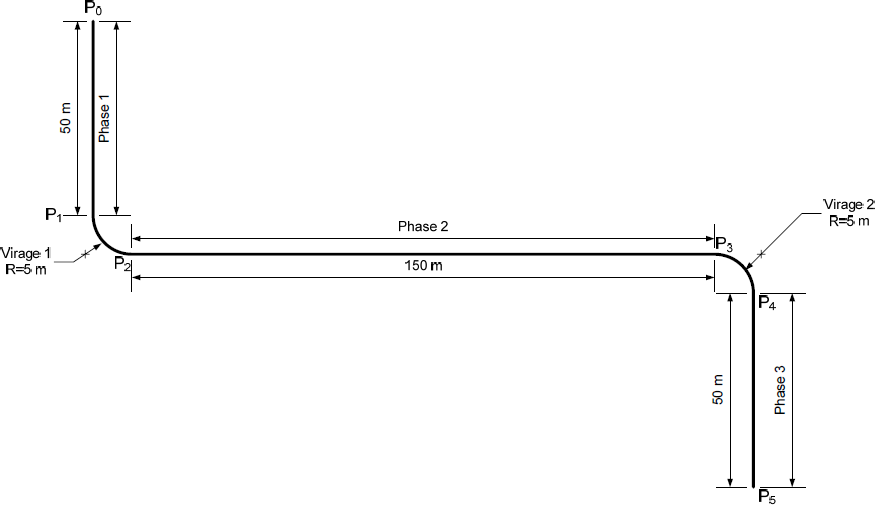
\includegraphics[width=.45\linewidth]{fig_25.png}
\caption{Résultat d’un essai de manoeuvre d’insertion avec l’algorithme d’aide au stationnement \label{fig_25}}
\end{figure}


\begin{figure}[H]
\centering
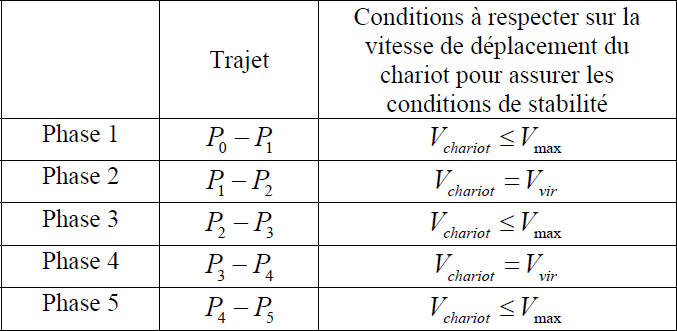
\includegraphics[width=\linewidth]{fig_26.png}
\caption{Extrait du diagramme des exigences du stationnement automatique \label{fig_26}}
\end{figure}


\begin{figure}[H]
\centering
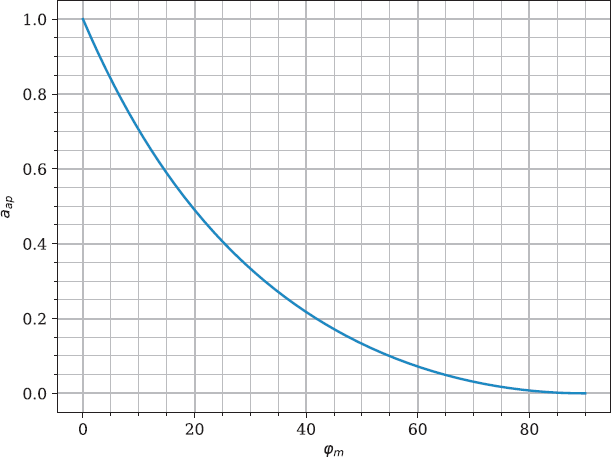
\includegraphics[width=.45\linewidth]{fig_27.png}
\caption{Extrait du diagramme des exigences du stationnement automatique \label{fig_27}}
\end{figure}


\begin{figure}[H]
\centering
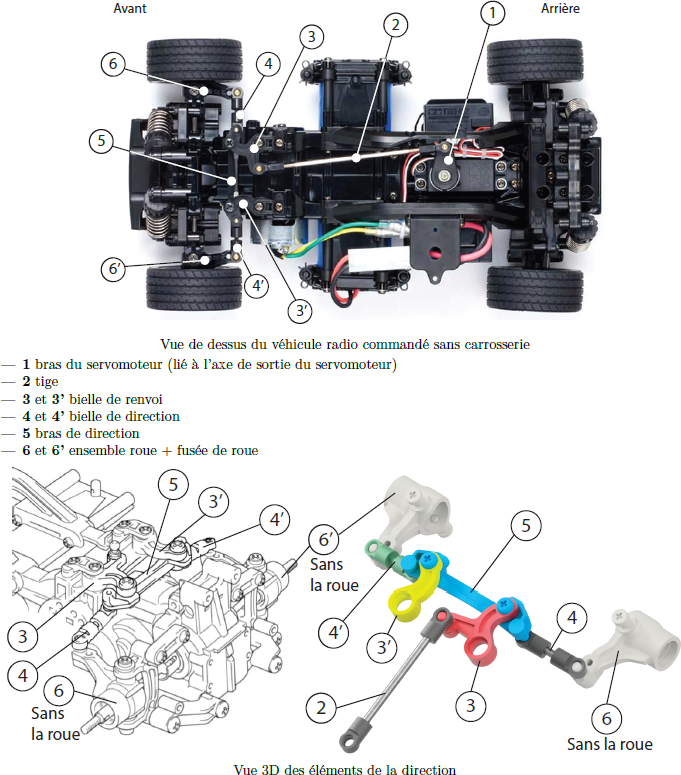
\includegraphics[width=.45\linewidth]{fig_28.png}
\caption{Description de la direction du véhicule radio commandé \label{fig_28}}
\end{figure}


\begin{figure}[H]
\centering
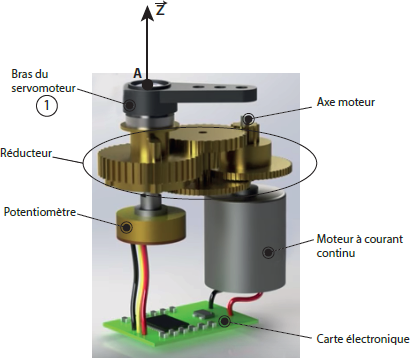
\includegraphics[width=.45\linewidth]{fig_29.png}
\caption{Composition du servomoteur \label{fig_29}}
\end{figure}